% ============================================================================
% SLIDE THUYẾT TRÌNH BTL ĐIỆN TOÁN ĐÁM MÂY (INT 3319 3) - TICKETRUSH
% Theme: Metropolis (16:9), 18 slide đầy đủ minh chứng thực tế trên AWS
% Biên dịch: pdflatex slides.tex (2 lần)
% ============================================================================
\documentclass[aspectratio=169,11pt]{beamer}

\usepackage[utf8]{inputenc}
\usepackage[T5]{fontenc}
\usepackage[vietnamese]{babel}
\usepackage{booktabs}
\usepackage{array}
\usepackage{graphicx}
\usepackage{tikz}
\usetikzlibrary{shapes.geometric,arrows.meta,positioning,fit,backgrounds}
\usepackage{xurl}

% ---- Giao diện Beamer kinh điển: Boadilla (chuẩn slide bài giảng ĐH) ----
\usetheme{Boadilla}
\usecolortheme{default}
\setbeamertemplate{navigation symbols}{}

\definecolor{uetblue}{HTML}{3333B3}
\definecolor{uetaccent}{HTML}{C2410C}
\definecolor{softbg}{HTML}{EFEFF8}
\definecolor{okgreen}{HTML}{15803D}

\title[TicketRush - INT 3319 3]{TicketRush: Hệ thống đăng ký và đặt vé sự kiện\\chịu tải đột biến trên AWS}
\author[Nhóm TicketRush]{Phan Huy Anh (24020024) $\cdot$ Nguyễn Tất Bình (24020042)\\
        Trần Đức Hoàng (24020141) $\cdot$ Nguyễn Văn Hiếu (24021478)}
\institute[UET - ĐHQGHN]{Học phần: INT 3319 3 - Điện toán đám mây \quad|\quad GVHD: Trần Trúc Mai, Nguyễn Xuân Trường\\
           Khoa Công nghệ Thông tin - Trường Đại học Công nghệ, ĐHQGHN\\[4pt]
           {\scriptsize\color{uetblue}\url{https://d3m6e24vu2nkwf.cloudfront.net} $\cdot$ \url{https://github.com/nguyenhieu21016/TicketRush}}}
\date[2026]{Hà Nội, 2026}

\begin{document}

% ============================================================================
% SLIDE 1: BÌA (Chuẩn Boadilla)
% ============================================================================
\begin{frame}[plain]
  \titlepage
\end{frame}

% ============================================================================
% SLIDE 2: NỘI DUNG TRÌNH BÀY
% ============================================================================
\begin{frame}{Nội dung trình bày}
  \begin{columns}[T]
    \column{0.48\textwidth}
    \begin{block}{Phần I - Bài toán \& Hạ tầng AWS}
      \small
      \begin{enumerate}
        \setlength{\itemsep}{6pt}
        \item Bài toán Flash-Sale \& Mục tiêu hệ thống
        \item Kiến trúc tổng thể 3 tầng + Serverless
        \item Mạng riêng VPC 2 AZ, Private EC2 \& Security Groups
        \item ALB, Auto Scaling Group \& CloudFront OAC
      \end{enumerate}
    \end{block}

    \column{0.48\textwidth}
    \begin{block}{Phần II - Dữ liệu, Ứng dụng \& Kiểm thử}
      \small
      \begin{enumerate}
        \setcounter{enumi}{4}
        \setlength{\itemsep}{6pt}
        \item CSDL RDS Multi-AZ, Redis TLS \& Lưu trữ đa loại
        \item Bảo mật IAM Role, Secrets Manager \& Ứng dụng
        \item Chống bán vượt số chỗ 3 lớp \& Pipeline SQS/Lambda
        \item Giám sát, Kiểm thử 600 Users, Chi phí \& Tổng kết
      \end{enumerate}
    \end{block}
  \end{columns}
\end{frame}

% ============================================================================
% SLIDE 3: BÀI TOÁN & MỤC TIÊU
% ============================================================================
\begin{frame}{1. Bài toán Flash-Sale \& Mục tiêu hệ thống}
  \begin{columns}[T]
    \column{0.48\textwidth}
    \begin{block}{Thách thức thực tế}
      \footnotesize
      \begin{itemize}
        \setlength{\itemsep}{4pt}
        \item \textbf{Tải đột biến:} Lưu lượng tăng hàng trăm lần trong vài phút mở bán, rồi giảm về gần 0 ngoài giờ cao điểm.
        \item \textbf{Bán vượt số chỗ (Overselling):} Tranh chấp ghi đồng thời (\textit{race condition}) vào CSDL.
        \item \textbf{Nghẽn tác vụ chậm:} Sinh ảnh mã QR và gửi email trực tiếp trong luồng HTTP gây timeout.
        \item \textbf{Lãng phí chi phí:} Duy trì cụm máy chủ cấu hình lớn cố định 24/7 chỉ để đón vài phút cao điểm.
      \end{itemize}
    \end{block}

    \column{0.48\textwidth}
    \begin{block}{Giải pháp TicketRush trên AWS}
      \footnotesize
      \begin{itemize}
        \setlength{\itemsep}{4pt}
        \item \textbf{Sẵn sàng cao \& Tự co giãn:} Kiến trúc 3 tầng trên 2 AZ, ALB + Auto Scaling (\texttt{Min 2 / Max 4}).
        \item \textbf{Chống bán lố 3 lớp:} Redis \texttt{DECRBY} + RDS Atomic \texttt{UPDATE} + \texttt{CHECK >= 0}.
        \item \textbf{Bất đồng bộ Serverless:} Tách tạo QR/S3/Email sang \textbf{SQS + DLQ + Lambda + DynamoDB}.
        \item \textbf{Bảo mật chuẩn Cloud:} Private Subnet, CloudFront OAC, IAM Role, Secrets Manager, TLS/AES-256.
      \end{itemize}
    \end{block}
  \end{columns}
\end{frame}

% ============================================================================
% SLIDE 4: ĐỐI CHIẾU 8 HẠNG MỤC BẮT BUỘC
% ============================================================================
\begin{frame}{2. Mức độ đáp ứng 8 hạng mục bắt buộc}
  \scriptsize
  \renewcommand{\arraystretch}{1.15}
  \begin{tabular}{@{} c >{\raggedright\arraybackslash}p{4.1cm} >{\raggedright\arraybackslash}p{7.8cm} c @{}}
    \toprule
    \textbf{\#} & \textbf{Hạng mục bắt buộc} & \textbf{Thành phần triển khai thực tế (\texttt{ap-southeast-1})} & \textbf{KQ} \\
    \midrule
    1 & VPC, public \& private subnet $\ge 2$ AZ & \texttt{ticketrush-vpc} (\texttt{10.0.0.0/16}), 6 subnet trên \texttt{1a/1b}, IGW, NAT GW & Đạt \\
    2 & Máy chủ ứng dụng Private Subnet & EC2 \texttt{t3.small} (ASG) trong \texttt{tr-app-a/b}, không Public IP, SG từ ALB & Đạt \\
    3 & $\ge 2$ loại lưu trữ khác nhau & S3 (\texttt{ticketrush-web}, \texttt{ticketrush-assets-hieu}), EBS \texttt{gp3} 20 GiB, DynamoDB & Đạt \\
    4 & Cơ sở dữ liệu quản trị sẵn & RDS MySQL 8.4 \textbf{Multi-AZ} (\texttt{db.t3.micro}) + ElastiCache Redis 7.1 TLS & Đạt \\
    5 & IAM Role, không hardcode key & \texttt{ticketrush-ec2-role}, \texttt{ticketrush-lambda-execution-role}, Secrets Manager & Đạt \\
    6 & Load Balancing \& Auto Scaling & \texttt{ticketrush-alb} + \texttt{ticketrush-asg} (Target Tracking \texttt{3000 req/target}) & Đạt \\
    7 & Giám sát \& $\ge 1$ cảnh báo thử & CloudWatch Dashboard \texttt{TicketRush}, 7 Alarms + email cảnh báo SNS & Đạt \\
    8 & Ước tính chi phí hàng tháng & Bảng chi phí chi tiết AWS Pricing (\textbf{$\approx$ \$196 - \$198/tháng}) & Đạt \\
    \bottomrule
  \end{tabular}
\end{frame}

% ============================================================================
% SLIDE 5: KIẾN TRÚC TỔNG THỂ
% ============================================================================
\begin{frame}{3. Kiến trúc tổng thể hệ thống trên AWS}
  \centering
  \resizebox{0.97\textwidth}{!}{%
  \begin{tikzpicture}[
    node distance=0.7cm and 0.85cm,
    box/.style={rectangle, rounded corners=4pt, draw=uetblue, fill=white, thick, align=center, font=\sffamily\footnotesize, minimum height=0.95cm, minimum width=2.3cm, inner sep=4pt},
    awsbox/.style={rectangle, rounded corners=4pt, draw=uetaccent, fill=orange!6, thick, align=center, font=\sffamily\footnotesize, minimum height=0.9cm, minimum width=2.6cm, inner sep=4pt},
    databox/.style={cylinder, shape border rotate=90, aspect=0.25, draw=uetblue, fill=blue!6, thick, align=center, font=\sffamily\footnotesize, minimum height=1.1cm, minimum width=2.3cm, inner sep=4pt},
    zone/.style={rectangle, rounded corners=6pt, dashed, draw=gray!70, inner sep=8pt},
    arrow/.style={-{Stealth[length=5.5pt]}, thick, color=uetblue},
    asyncarrow/.style={-{Stealth[length=5.5pt]}, thick, dashed, color=uetaccent}
  ]
    \node[box, fill=gray!10, minimum width=2.0cm] (user) {\textbf{Người dùng}\\(Trình duyệt)};
    \node[awsbox, right=1.0cm of user, minimum width=2.7cm] (cf) {\textbf{CloudFront CDN}\\{\scriptsize\texttt{E3K3I9C6DRVNO7}}\\HTTPS + OAC};
    \node[awsbox, below=0.8cm of cf, minimum width=2.7cm] (s3web) {\textbf{S3 Frontend}\\{\scriptsize\texttt{ticketrush-web}}\\Private OAC};

    \node[box, fill=green!7, draw=okgreen, right=1.9cm of cf, minimum width=2.9cm] (alb) {\textbf{ALB}\\{\scriptsize\texttt{ticketrush-alb}}\\Public (1a / 1b)};
    \node[box, fill=green!5, draw=okgreen, below=0.55cm of alb, minimum width=2.9cm] (nat) {\textbf{NAT Gateway}\\{\scriptsize\texttt{tr-public-a}}};

    \node[box, fill=blue!5, right=1.2cm of alb, yshift=0.3cm, minimum width=3.0cm] (ec2a) {\textbf{EC2 (AZ 1a) - ASG}\\{\scriptsize\texttt{t3.small}} + EBS 20GB\\FastAPI (:8000)};
    \node[box, fill=blue!5, below=0.45cm of ec2a, minimum width=3.0cm] (ec2b) {\textbf{EC2 (AZ 1b) - ASG}\\{\scriptsize\texttt{t3.small}} + EBS 20GB\\FastAPI (:8000)};

    \node[databox, below=1.45cm of ec2b, xshift=-1.55cm] (rds) {\textbf{RDS MySQL 8.4}\\Multi-AZ (1a/1b)\\\texttt{db.t3.micro}};
    \node[databox, right=0.75cm of rds] (redis) {\textbf{ElastiCache Redis}\\7.1 TLS (:6379)\\\texttt{cache.t3.micro}};

    \node[awsbox, right=1.8cm of ec2a, yshift=0.2cm] (sqs) {\textbf{SQS + DLQ}\\{\scriptsize\texttt{ticket-generation}}\\MaxReceive=3};
    \node[awsbox, below=0.55cm of sqs] (lambda) {\textbf{AWS Lambda}\\Python 3.11 (512MB)\\QR + Idempotency};
    \node[awsbox, below=0.55cm of lambda] (s3qr) {\textbf{S3 Assets \& DynamoDB}\\{\scriptsize\texttt{ticketrush-assets-hieu}}\\{\scriptsize\texttt{ticket-idempotency}}};
    \node[awsbox, below=0.55cm of s3qr] (mail) {\textbf{Gmail SMTP / SES}\\Gửi vé QR tới\\khách hàng};

    \begin{scope}[on background layer]
      \node[zone, draw=okgreen!70, fill=green!2, fit=(alb)(nat), label={[font=\sffamily\scriptsize\bfseries, text=okgreen]above:Public Subnets}] (pubzone) {};
      \node[zone, draw=uetblue!80, fill=blue!2, fit=(ec2a)(ec2b), label={[font=\sffamily\scriptsize\bfseries, text=uetblue]above:Private App Subnets (ASG 2-4)}] (appzone) {};
      \node[zone, draw=uetblue!70, fill=cyan!3, fit=(rds)(redis), label={[font=\sffamily\scriptsize\bfseries, text=uetblue]below:Private Data Subnets}] (datazone) {};
      \node[zone, draw=black!75, line width=1pt, solid, fit=(pubzone)(appzone)(datazone), inner xsep=12pt, inner ysep=18pt] (vpcbox) {};
      \node[font=\sffamily\footnotesize\bfseries, fill=white, inner sep=2pt, anchor=south] at (vpcbox.north) {VPC \texttt{ticketrush-vpc} (10.0.0.0/16 - \texttt{ap-southeast-1})};
    \end{scope}

    \node[box, fill=purple!6, draw=purple, below=0.85cm of s3web, minimum width=2.7cm] (cw) {\textbf{CloudWatch + SNS}\\Dashboard \& 7 Alarms};
    \node[box, fill=purple!6, draw=purple, below=0.45cm of cw, minimum width=2.7cm] (iam) {\textbf{IAM Roles \& Secrets}\\{\scriptsize\texttt{ticketrush-ec2-role}}};

    \draw[arrow] (user) -- node[above, font=\scriptsize]{HTTPS} (cf);
    \draw[arrow] (cf) -- node[right, font=\scriptsize]{OAC} (s3web);
    \draw[arrow] (cf) -- node[above, font=\scriptsize, fill=white, inner sep=1pt]{\texttt{/api/*}} (alb);
    \draw[arrow] (alb.east) -- ++(0.45,0) |- (ec2a.west);
    \draw[arrow] (alb.east) -- ++(0.45,0) |- (ec2b.west);
    \draw[arrow] (ec2b.south) -- ++(0,-0.55) -| (rds.north) node[pos=0.25, above, font=\scriptsize, fill=white, inner sep=1pt]{:3306};
    \draw[arrow] (ec2b.south) -- ++(0,-0.55) -| (redis.north) node[pos=0.25, above, font=\scriptsize, fill=white, inner sep=1pt]{:6379 TLS};
    \draw[asyncarrow] (ec2a.east) -- node[above, font=\scriptsize, fill=white, inner sep=1pt]{Push} (sqs.west);
    \draw[asyncarrow] (sqs) -- (lambda);
    \draw[asyncarrow] (lambda) -- (s3qr);
    \draw[asyncarrow] (s3qr) -- (mail);
    \draw[asyncarrow, color=purple] (cw.east) -- (cw.east -| vpcbox.west);
    \draw[asyncarrow, color=purple] (iam.east) -- (iam.east -| vpcbox.west);
  \end{tikzpicture}
  }
\end{frame}

% ============================================================================
% SLIDE 6: MẠNG RIÊNG VPC 2 AZ
% ============================================================================
\begin{frame}{4. Thiết kế mạng riêng VPC 3 tầng trên 2 AZ}
  \begin{columns}[c]
    \column{0.42\textwidth}
    \footnotesize
    \begin{itemize}
      \setlength{\itemsep}{4pt}
      \item \textbf{VPC \texttt{ticketrush-vpc}} (\texttt{10.0.0.0/16}) trải trên 2 vùng sẵn sàng \texttt{ap-southeast-1a} và \texttt{1b}.
      \item \textbf{2 Public Subnets} (\texttt{10.0.1.0/24}, \texttt{10.0.2.0/24}): đặt ALB, NAT Gateway; route \texttt{0.0.0.0/0 $\rightarrow$ IGW}.
      \item \textbf{2 Private App Subnets} (\texttt{10.0.11.0/24}, \texttt{10.0.12.0/24}): đặt EC2 ASG; ra ngoài qua NAT GW.
      \item \textbf{2 Private Data Subnets} (\texttt{10.0.21.0/24}, \texttt{10.0.22.0/24}): cô lập hoàn toàn RDS Multi-AZ \& Redis (chỉ có route \texttt{local}).
    \end{itemize}

    \column{0.56\textwidth}
    \centering
    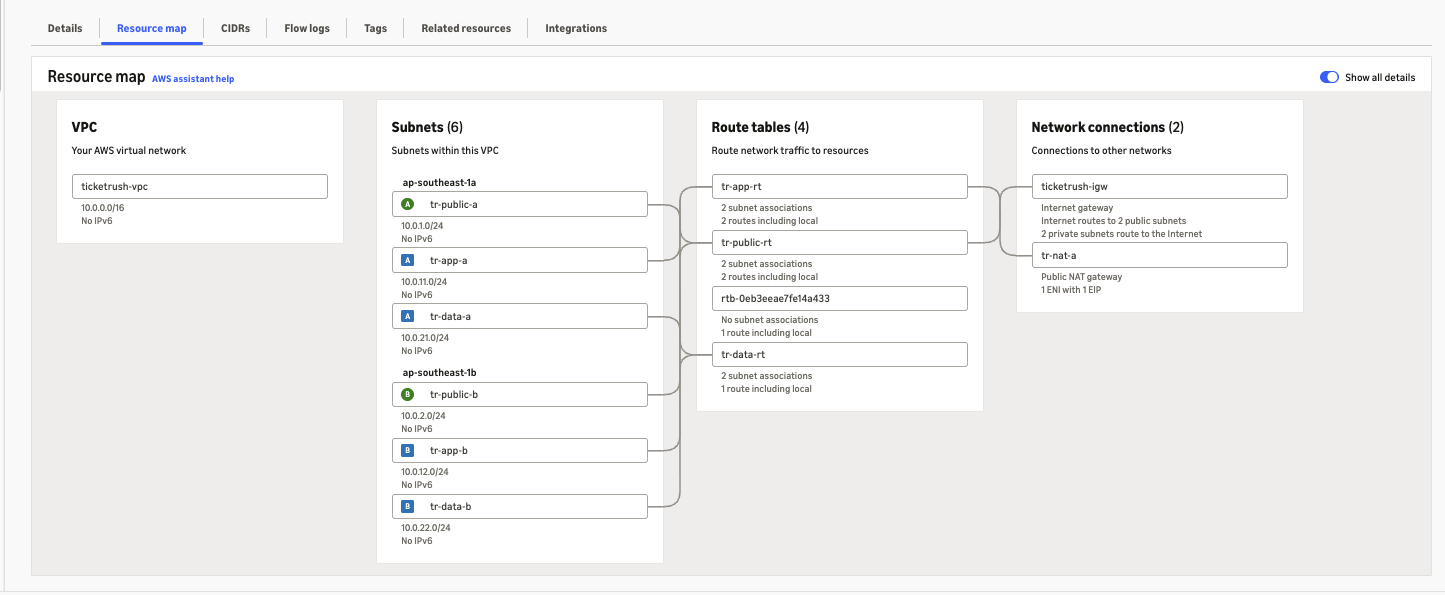
\includegraphics[width=\textwidth,height=0.72\textheight,keepaspectratio]{images/vpc_subnets.png}\\[4pt]
    {\scriptsize Sơ đồ tài nguyên VPC \texttt{ticketrush-vpc} trên AWS Console}
  \end{columns}
\end{frame}

% ============================================================================
% SLIDE 7: CÔ LẬP PRIVATE EC2 & SECURITY GROUP CHAINING
% ============================================================================
\begin{frame}{5. Cô lập EC2 trong Private Subnet \& Security Group Chaining}
  \begin{columns}[c]
    \column{0.42\textwidth}
    \footnotesize
    \begin{itemize}
      \setlength{\itemsep}{5pt}
      \item \textbf{Không phơi máy chủ ra Internet:} Toàn bộ EC2 do ASG quản lý không có Public IPv4; máy mẫu \texttt{ticketrush-backend} luôn ở trạng thái \texttt{Stopped} khi vận hành.
      \item \textbf{Chuỗi Security Groups phân tầng:}
        \begin{itemize}\scriptsize
          \item \texttt{tr-alb-sg}: nhận HTTP cổng \texttt{80} từ Internet.
          \item \texttt{tr-app-sg}: cổng \texttt{8000} chỉ nhận lưu lượng từ \texttt{tr-alb-sg}.
          \item \texttt{tr-data-sg}: cổng \texttt{3306} \& \texttt{6379} chỉ nhận từ \texttt{tr-app-sg}.
        \end{itemize}
    \end{itemize}

    \column{0.56\textwidth}
    \centering
    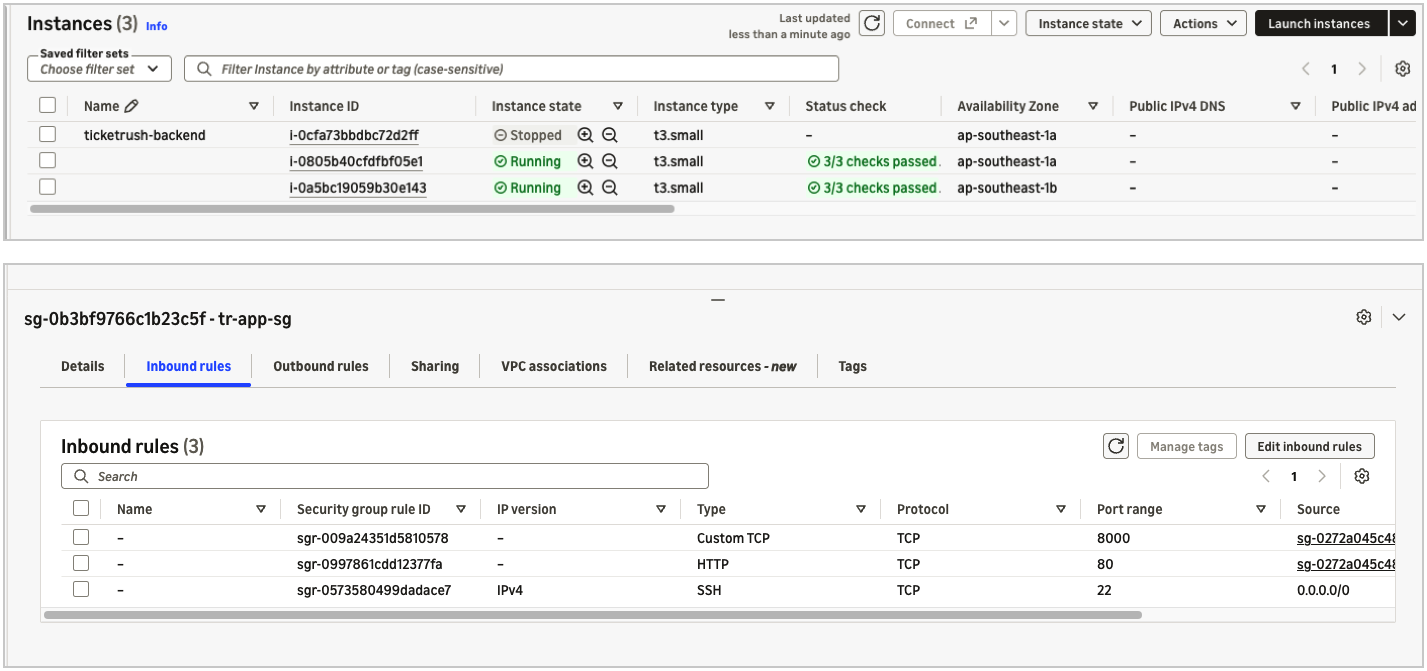
\includegraphics[width=\textwidth,height=0.74\textheight,keepaspectratio]{images/ec2_private_sg.png}
  \end{columns}
\end{frame}

% ============================================================================
% SLIDE 8: ALB, AUTO SCALING & CLOUDFRONT OAC
% ============================================================================
\begin{frame}{6. Cân bằng tải, Auto Scaling \& CloudFront CDN OAC}
  \begin{columns}[c]
    \column{0.46\textwidth}
    \footnotesize
    \begin{itemize}
      \setlength{\itemsep}{4pt}
      \item \textbf{CloudFront (\texttt{E3K3I9C6DRVNO7}):}
        \begin{itemize}\scriptsize
          \item \texttt{Default (*)}: S3 \texttt{ticketrush-web} qua \textbf{OAC} (chặn truy cập S3 trực tiếp, tự động redirect HTTPS).
          \item \texttt{/api/*}: chuyển tiếp không cache về ALB, tránh lỗi Mixed Content \& CORS.
        \end{itemize}
      \item \textbf{ALB + Auto Scaling Group:}
        \begin{itemize}\scriptsize
          \item \texttt{ticketrush-asg}: \textbf{Min 2 / Max 4} EC2 \texttt{t3.small}, Health Check \texttt{ELB (/health)}.
          \item \textbf{Target Tracking:} \texttt{ALBRequestCountPerTarget = 3000}, warmup 60s.
          \item \textbf{Golden AMI:} Đóng gói sẵn Docker image giúp máy mới lên sẵn sàng chỉ sau \textbf{65 giây}.
        \end{itemize}
    \end{itemize}

    \column{0.52\textwidth}
    \centering
    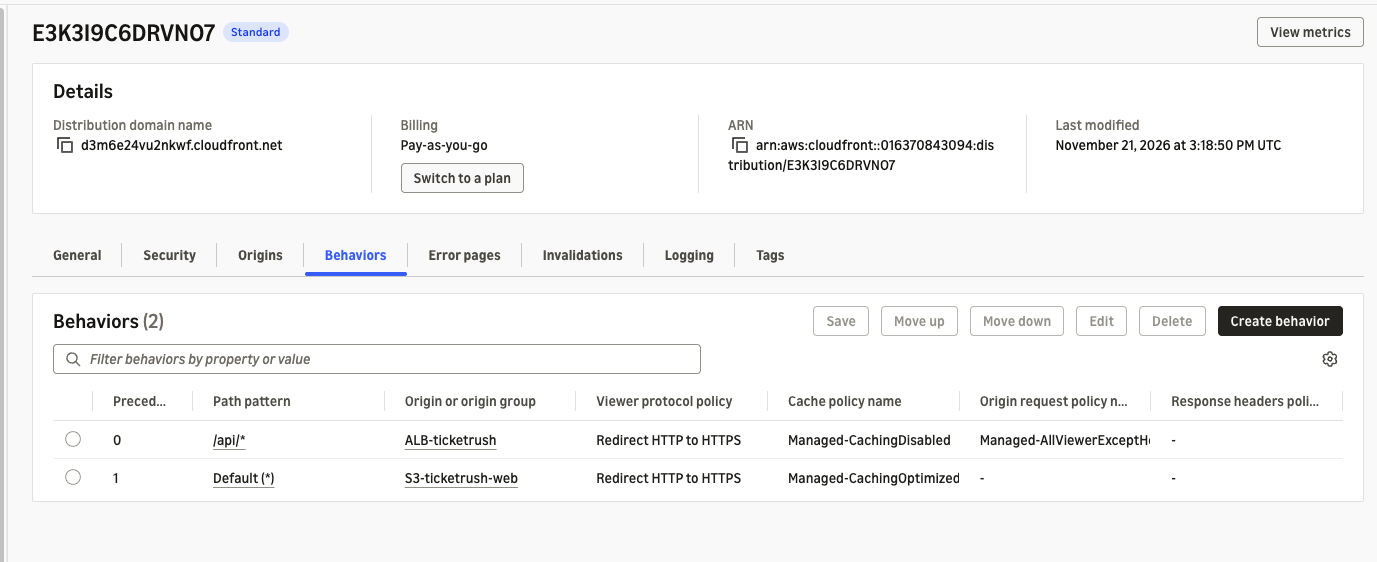
\includegraphics[width=\textwidth,height=0.70\textheight,keepaspectratio]{images/cloudfront_oac.png}\\[4pt]
    {\scriptsize Cấu hình 2 Behaviors trên CloudFront \texttt{E3K3I9C6DRVNO7}}
  \end{columns}
\end{frame}

% ============================================================================
% SLIDE 9: RDS MYSQL 8.4 MULTI-AZ & TỐI ƯU POOL
% ============================================================================
\begin{frame}{7. Amazon RDS MySQL 8.4 Multi-AZ \& Tối ưu kết nối}
  \begin{columns}[c]
    \column{0.46\textwidth}
    \footnotesize
    \begin{itemize}
      \setlength{\itemsep}{4pt}
      \item \textbf{RDS \texttt{ticketrush-mysql}:} Engine MySQL \texttt{8.4.11}, lớp \texttt{db.t3.micro}, \textbf{Multi-AZ = Yes} (\texttt{1a/1b}), \textbf{Public = No}, ổ 20 GiB \texttt{gp3}, backup tự động 7 ngày (PITR).
      \item \textbf{Lược đồ 4 bảng chuẩn hóa:} \texttt{users}, \texttt{events}, \texttt{bookings}, \texttt{tickets} với khóa ngoại và ràng buộc \texttt{CHECK >= 0} trên 3 hạng vé.
      \item \textbf{Đồng bộ Connection Pool với ASG:}
        \begin{itemize}\scriptsize
          \item Giới hạn SQLAlchemy \texttt{pool\_size=4, max\_overflow=2} (6 kết nối/worker).
          \item Ở đỉnh 4 EC2 (8 workers): $4 \times 2 \times 6 = \mathbf{48 < 64}$ trần kết nối của \texttt{db.t3.micro}, chừa $\ge 15$ kết nối cho Lambda \& quản trị.
        \end{itemize}
    \end{itemize}

    \column{0.52\textwidth}
    \centering
    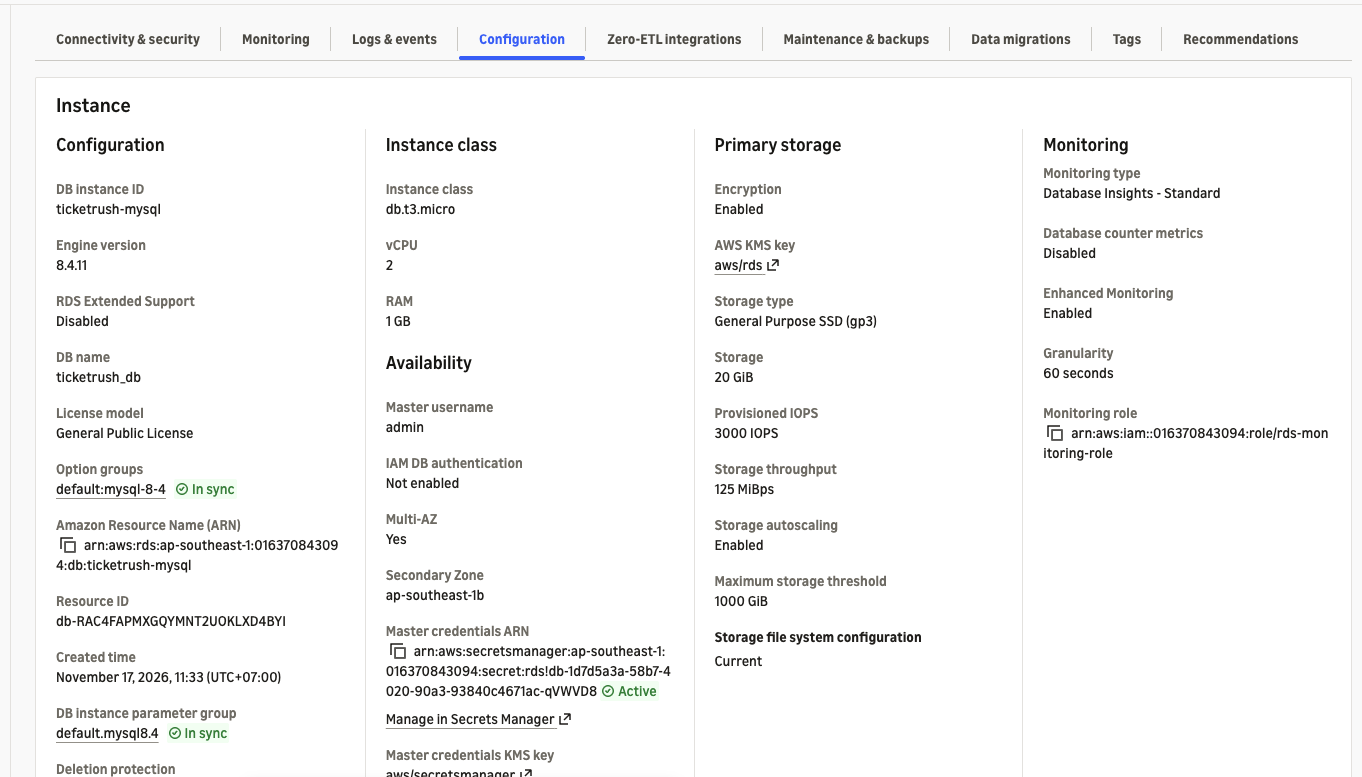
\includegraphics[width=\textwidth,height=0.74\textheight,keepaspectratio]{images/rds_multiaz.png}
  \end{columns}
\end{frame}

% ============================================================================
% SLIDE 10: REDIS TLS & LƯU TRỮ ĐA LOẠI
% ============================================================================
\begin{frame}{8. ElastiCache Redis 7.1 TLS \& Lưu trữ đa loại}
  \begin{columns}[c]
    \column{0.48\textwidth}
    \footnotesize
    \begin{itemize}
      \setlength{\itemsep}{4pt}
      \item \textbf{ElastiCache Redis (\texttt{ticketrush-redis-001}):} Redis \texttt{7.1.0}, \texttt{cache.t3.micro}, bật \textbf{TLS} \& \textbf{At-Rest}, đảm nhận 3 vai trò:
        \begin{itemize}\scriptsize
          \item Giữ chỗ nguyên tử \texttt{DECRBY} + TTL 600s.
          \item Cache-Aside danh sách sự kiện (tự invalidate khi thay đổi).
          \item Rate Limiting chống spam 10 req/60s (\texttt{HTTP 429}).
        \end{itemize}
      \item \textbf{3 loại lưu trữ chuyên biệt:}
        \begin{itemize}\scriptsize
          \item \textbf{Object (S3):} \texttt{ticketrush-web} (OAC) \& \texttt{ticketrush-assets-hieu} (poster công khai, QR riêng tư AES-256).
          \item \textbf{Block (EBS):} 20 GiB \texttt{gp3} (3.000 IOPS) gắn từng EC2.
          \item \textbf{NoSQL (DynamoDB):} Bảng chống trùng \texttt{PAY\_PER\_REQUEST}, TTL 24h.
        \end{itemize}
    \end{itemize}

    \column{0.50\textwidth}
    \centering
    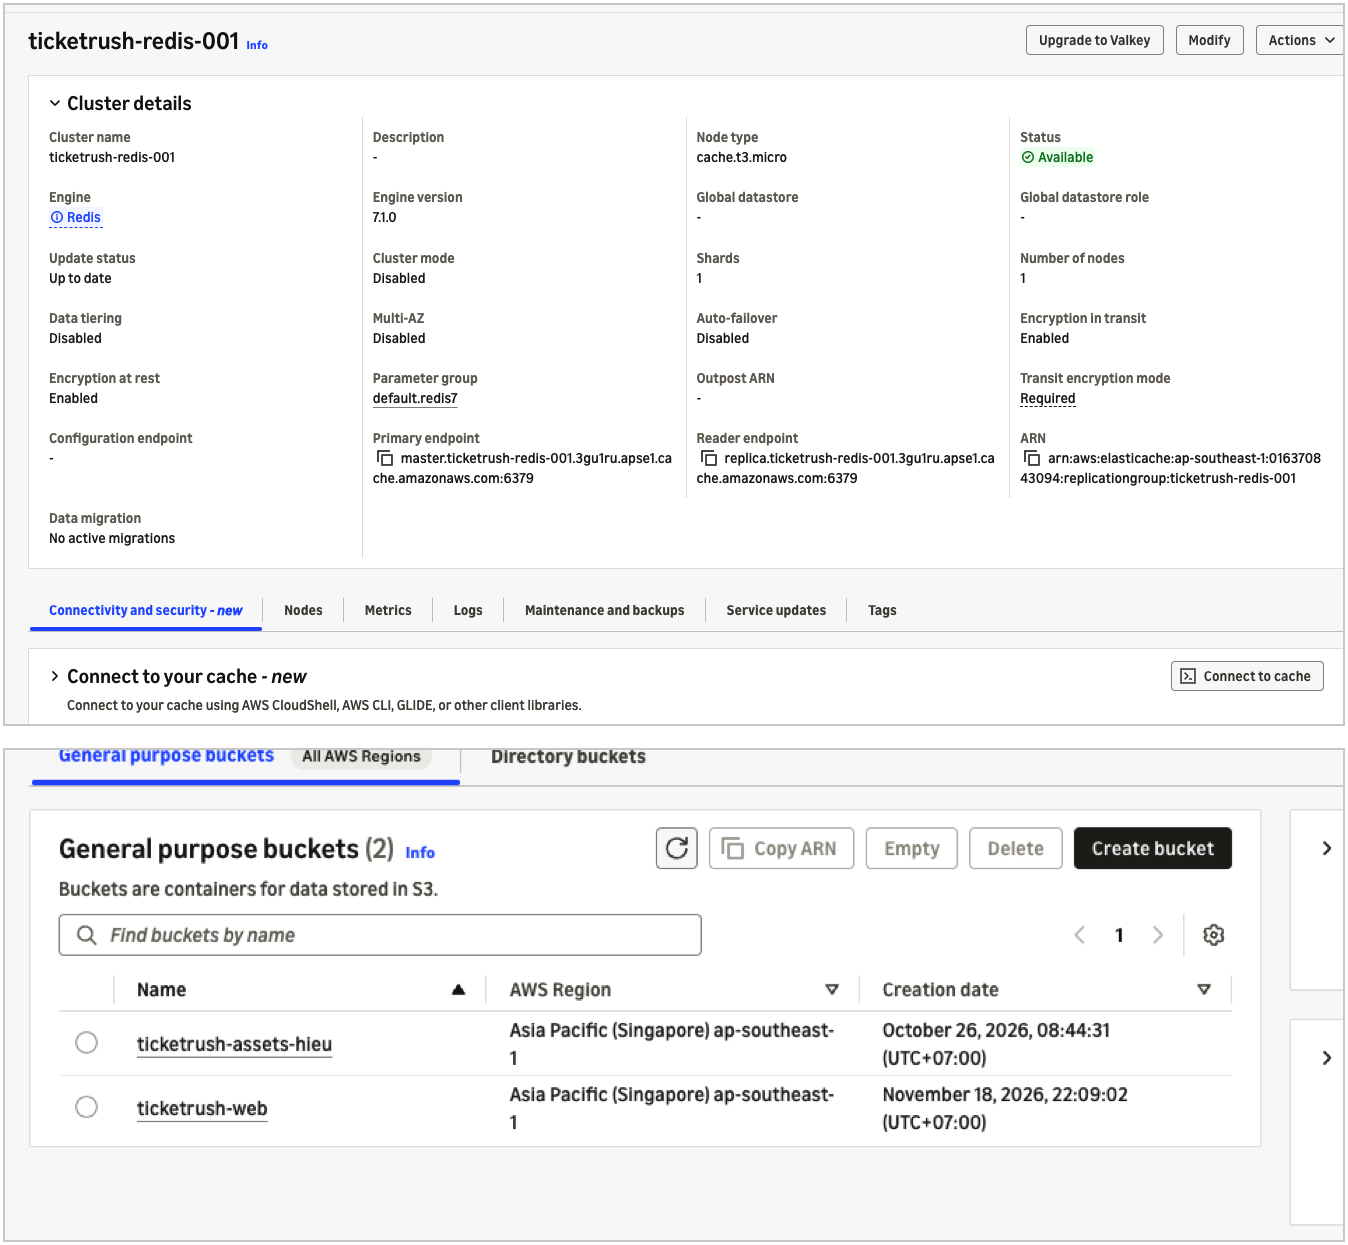
\includegraphics[width=\textwidth,height=0.74\textheight,keepaspectratio]{images/redis_s3.png}
  \end{columns}
\end{frame}

% ============================================================================
% SLIDE 11: BẢO MẬT & PHÂN QUYỀN IAM
% ============================================================================
\begin{frame}{9. Bảo mật, Phân quyền IAM \& Quản lý bí mật}
  \begin{columns}[c]
    \column{0.46\textwidth}
    \footnotesize
    \begin{itemize}
      \setlength{\itemsep}{4pt}
      \item \textbf{Không nhúng AWS Access Key:}
        \begin{itemize}\scriptsize
          \item EC2 gắn IAM Role \texttt{ticketrush-ec2-role} (SQS, SSM, inline \texttt{TicketRushS3AssetsAccess}).
          \item Lambda gắn \texttt{ticketrush-lambda-execution-role}.
        \end{itemize}
      \item \textbf{AWS Secrets Manager:} Khởi tạo và quản lý mật khẩu quản trị RDS tập trung, tách biệt khỏi mã nguồn GitHub.
      \item \textbf{Mã hóa đường truyền \& lưu trữ:} HTTPS (CloudFront), Redis TLS (\texttt{rediss://}), SMTP STARTTLS, S3 SSE-S3 (\texttt{AES256}).
      \item \textbf{Bảo mật ứng dụng:} Mật khẩu \textbf{bcrypt}, phiên \textbf{JWT}, phân quyền RBAC (\texttt{USER/ADMIN}), chống SQL Injection (ORM/parameterized).
    \end{itemize}

    \column{0.52\textwidth}
    \centering
    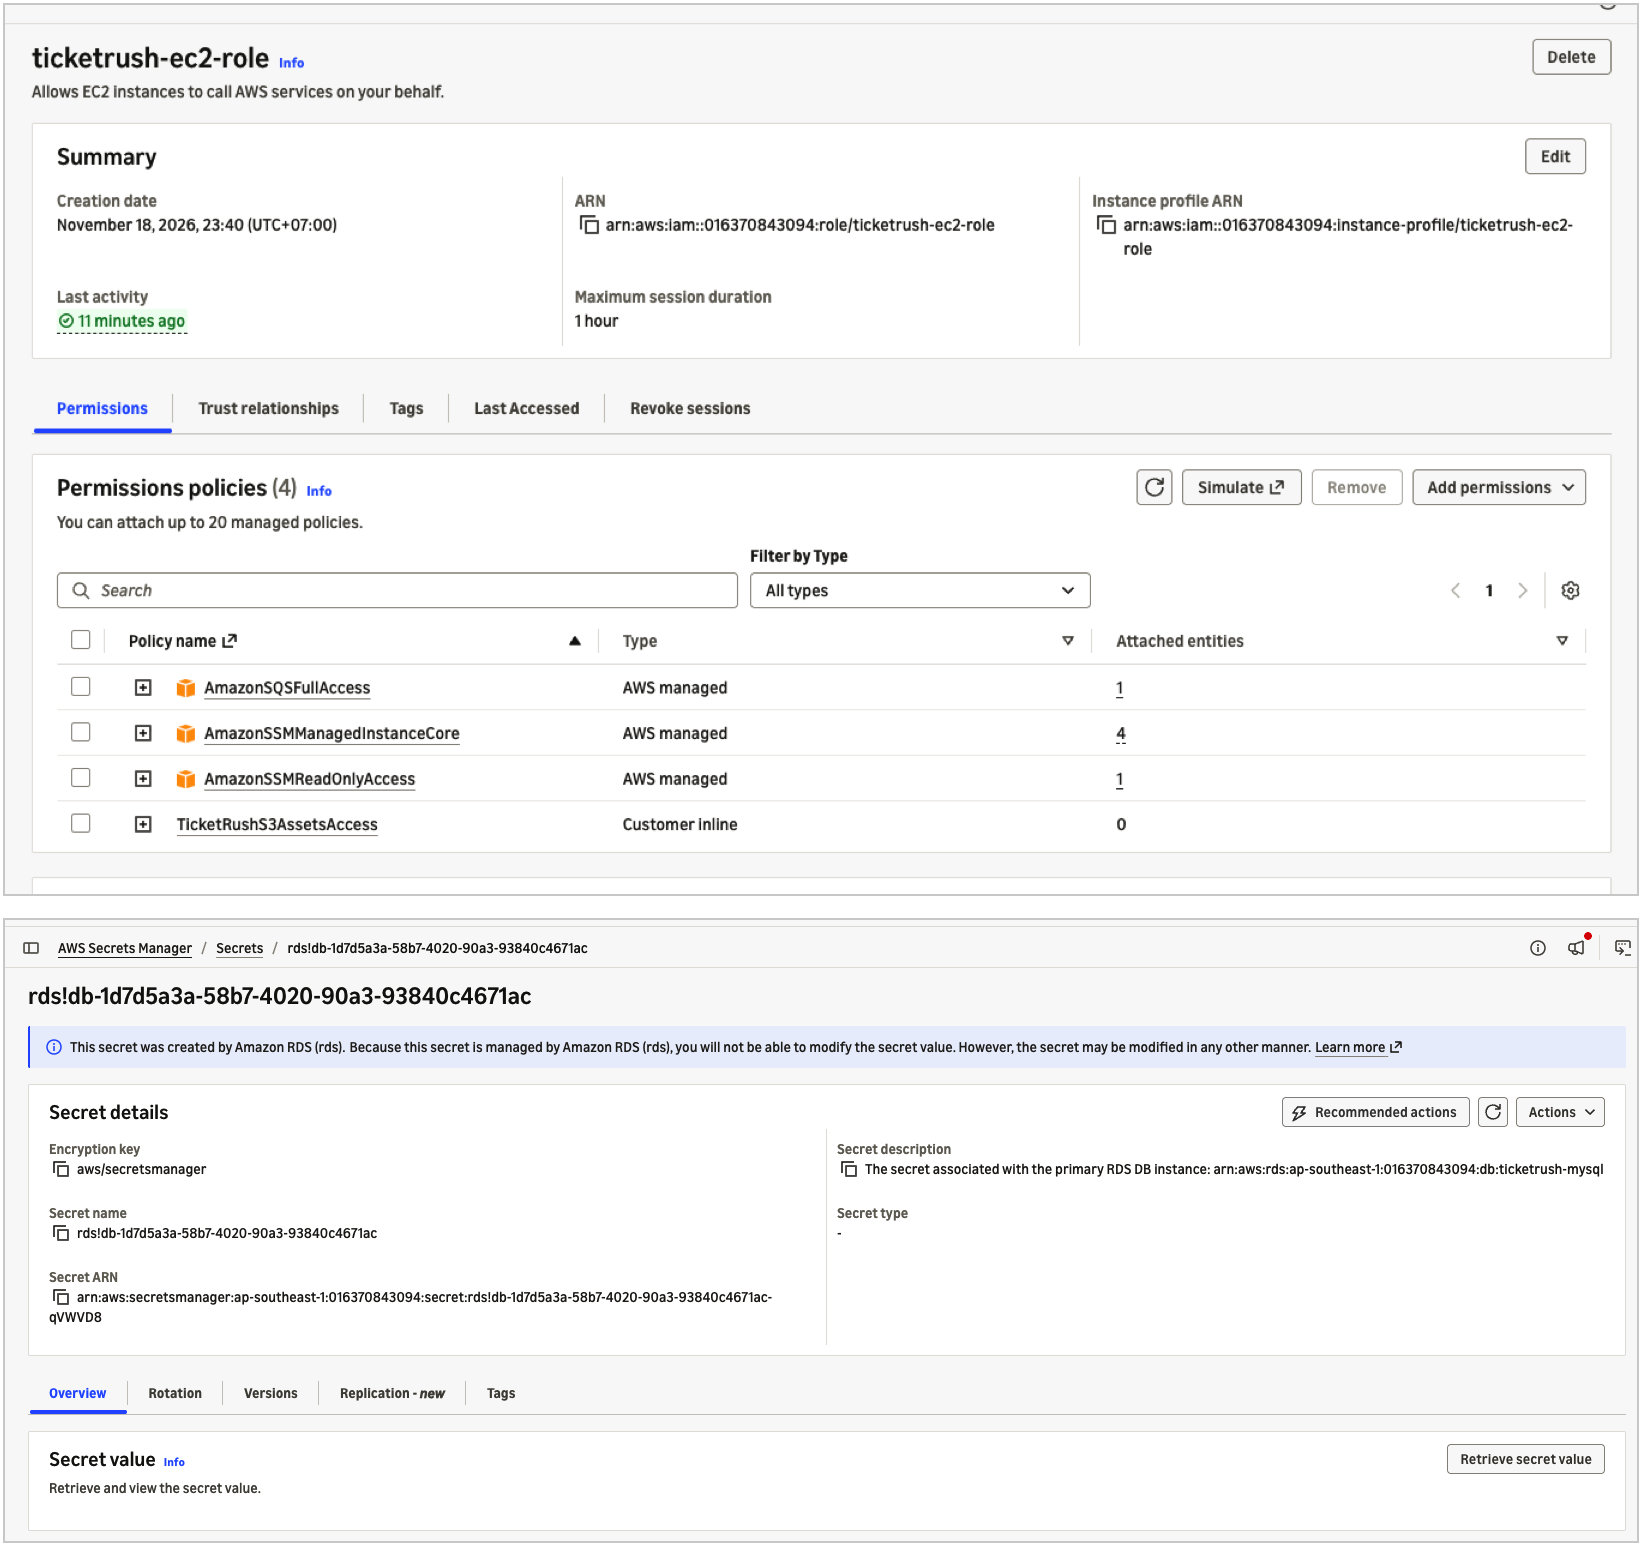
\includegraphics[width=\textwidth,height=0.74\textheight,keepaspectratio]{images/iam_secrets.png}
  \end{columns}
\end{frame}

% ============================================================================
% SLIDE 12: CHỐNG BÁN VƯỢT SỐ CHỖ & PIPELINE BẤT ĐỒNG BỘ
% ============================================================================
\begin{frame}{10. Chống bán vượt số chỗ (3 lớp) \& Pipeline bất đồng bộ}
  \centering
  \resizebox{0.96\textwidth}{!}{%
  \begin{tikzpicture}[
    node distance=0.55cm and 0.7cm,
    stepbox/.style={rectangle, rounded corners=4pt, draw=uetblue, fill=blue!4, thick, align=center, font=\sffamily\footnotesize, minimum width=2.7cm, minimum height=0.85cm, inner sep=4pt},
    dec/.style={diamond, draw=uetaccent, fill=orange!6, thick, align=center, font=\sffamily\scriptsize, aspect=2.1, inner sep=2pt},
    errbox/.style={rectangle, rounded corners=3pt, draw=red!70!black, fill=red!6, font=\sffamily\scriptsize, align=center, minimum width=2.3cm, inner sep=4pt},
    okbox/.style={rectangle, rounded corners=4pt, draw=okgreen, fill=green!7, thick, align=center, font=\sffamily\footnotesize, minimum width=3.0cm, inner sep=4pt},
    arr/.style={-{Stealth[length=5pt]}, thick, color=uetblue}
  ]
    \node[stepbox] (req) {\textbf{POST /reserve}\\(JWT + Rate Limit)};
    \node[dec, right=0.8cm of req] (rl) {Vượt 10/60s?};
    \node[stepbox, right=0.95cm of rl] (redis) {\textbf{Lớp 1: Redis DECRBY}\\Hold TTL 600s};
    \node[dec, right=0.8cm of redis] (hasseat) {Còn ghế?};
    \node[stepbox, right=0.95cm of hasseat] (confirm) {\textbf{Lớp 2 \& 3: RDS}\\Atomic UPDATE + CHECK};

    \node[errbox, below=0.7cm of rl] (e429) {\textbf{HTTP 429}\\Too Many Req};
    \node[errbox, below=0.7cm of hasseat] (e409) {\textbf{INCRBY hoàn vé}\\HTTP 409 Hết vé};
    \node[okbox, below=0.7cm of confirm] (sqs) {\textbf{Xóa Cache \& Đẩy SQS}\\Trả HTTP 200 tức thì};
    \node[okbox, below=0.65cm of sqs, fill=orange!7, draw=uetaccent] (lam) {\textbf{Lambda + DynamoDB}\\QR $\rightarrow$ S3 \& Gửi Email};

    \draw[arr] (req) -- (rl);
    \draw[arr] (rl) -- node[right, font=\scriptsize]{Có} (e429);
    \draw[arr] (rl) -- node[above, font=\scriptsize]{Không} (redis);
    \draw[arr] (redis) -- (hasseat);
    \draw[arr] (hasseat) -- node[right, font=\scriptsize]{Không} (e409);
    \draw[arr] (hasseat) -- node[above, font=\scriptsize]{Có} (confirm);
    \draw[arr] (confirm) -- (sqs);
    \draw[arr, dashed, color=uetaccent] (sqs) -- node[right, font=\scriptsize, text=uetaccent]{Async (DLQ max 3)} (lam);
  \end{tikzpicture}
  }\\[8pt]
  \begin{columns}[T]
    \column{0.48\textwidth}
    \footnotesize
    \textbf{Phòng vệ 3 lớp:} Chặn nhanh trên RAM Redis (\texttt{DECRBY}) $\rightarrow$ trừ nguyên tử mức hàng trên RDS InnoDB $\rightarrow$ ràng buộc \texttt{CHECK >= 0}.
    \column{0.48\textwidth}
    \footnotesize
    \textbf{Serverless Worker:} Lambda (\texttt{Python 3.11, 512MB, 60s}) chống trùng qua DynamoDB, sinh QR lưu S3 AES-256 và gửi email kèm ảnh đính kèm.
  \end{columns}
\end{frame}

% ============================================================================
% SLIDE 13: GIAO DIỆN NGƯỜI DÙNG & EMAIL VÉ QR
% ============================================================================
\begin{frame}{11. Giao diện đặt vé, Email QR \& Admin Check-in}
  \begin{columns}[c]
    \column{0.49\textwidth}
    \centering
    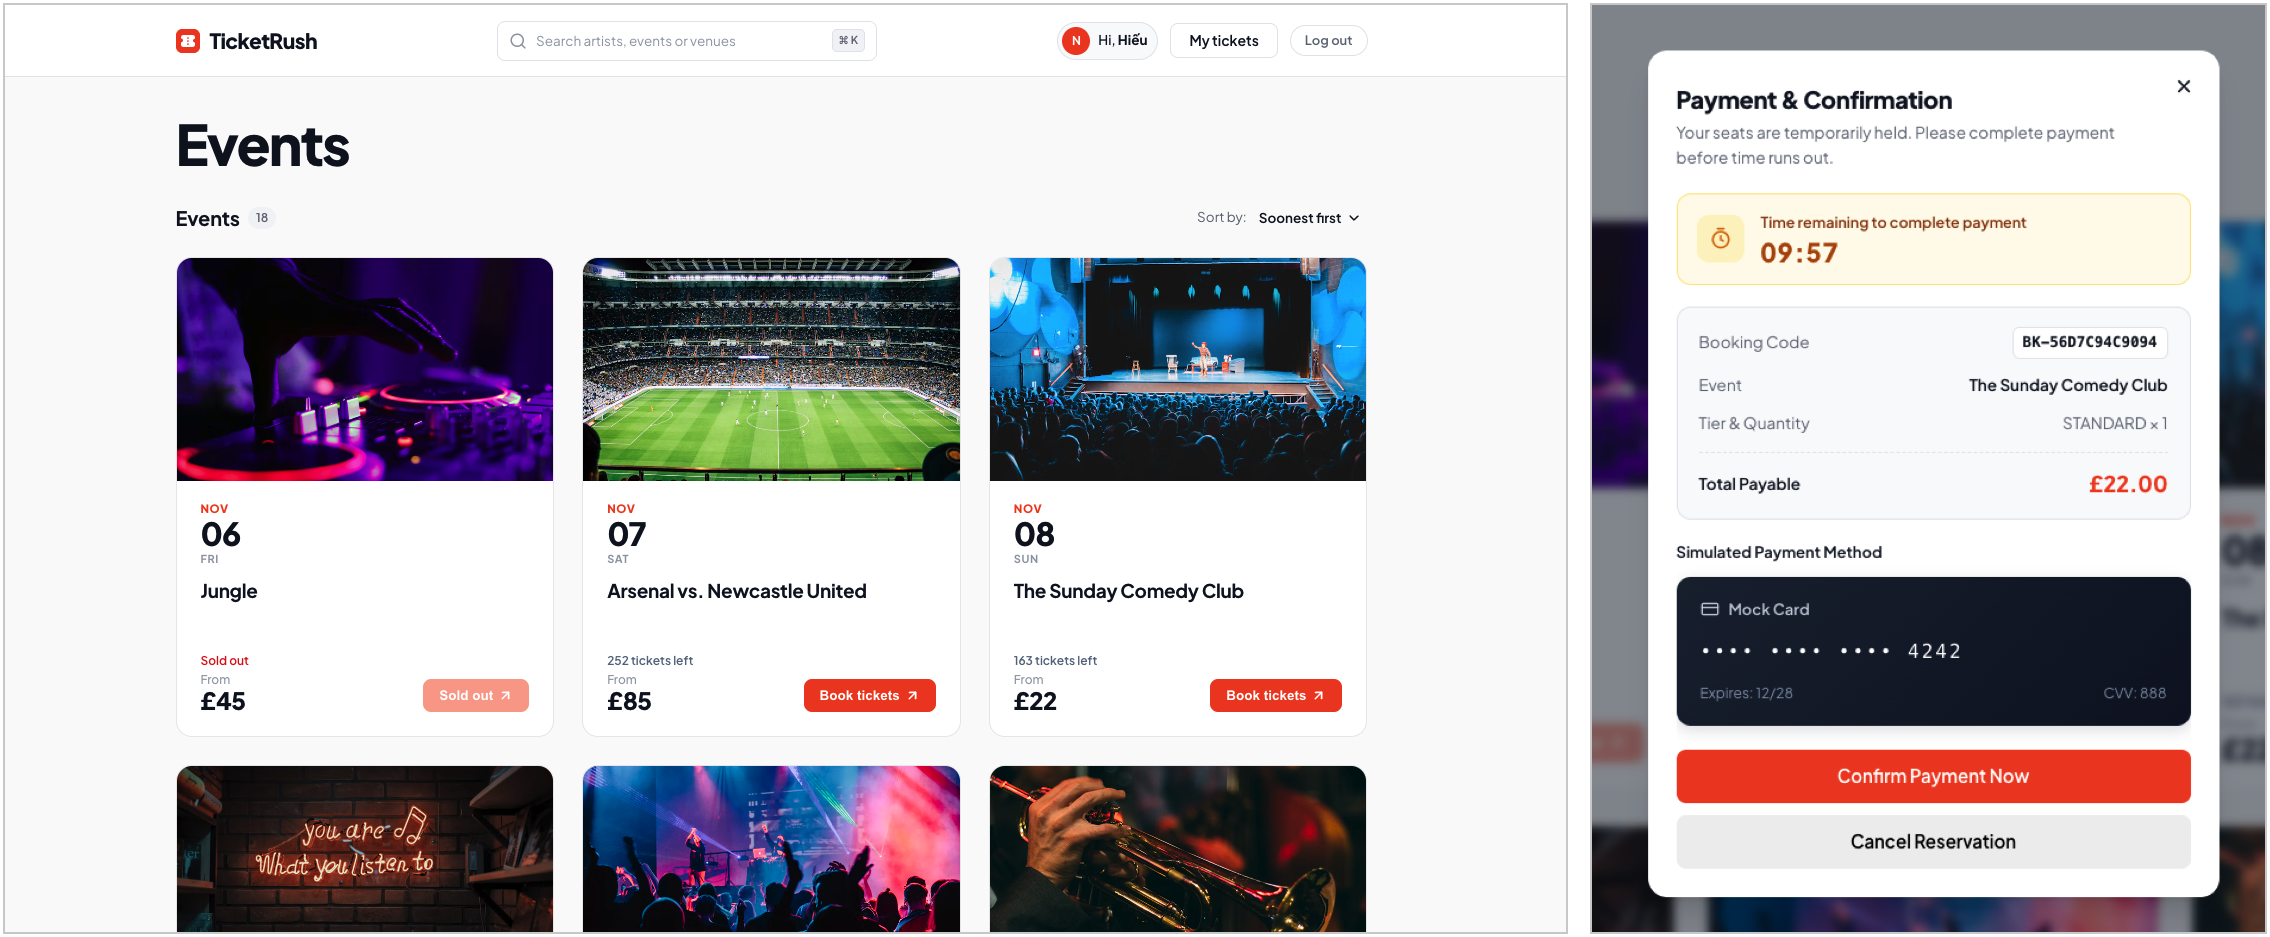
\includegraphics[width=\textwidth,height=0.31\textheight,keepaspectratio]{images/ui_booking_checkout.png}\\[2pt]
    {\tiny Giao diện HTTPS CloudFront \& Modal giữ chỗ TTL 10 phút}\\[5pt]
    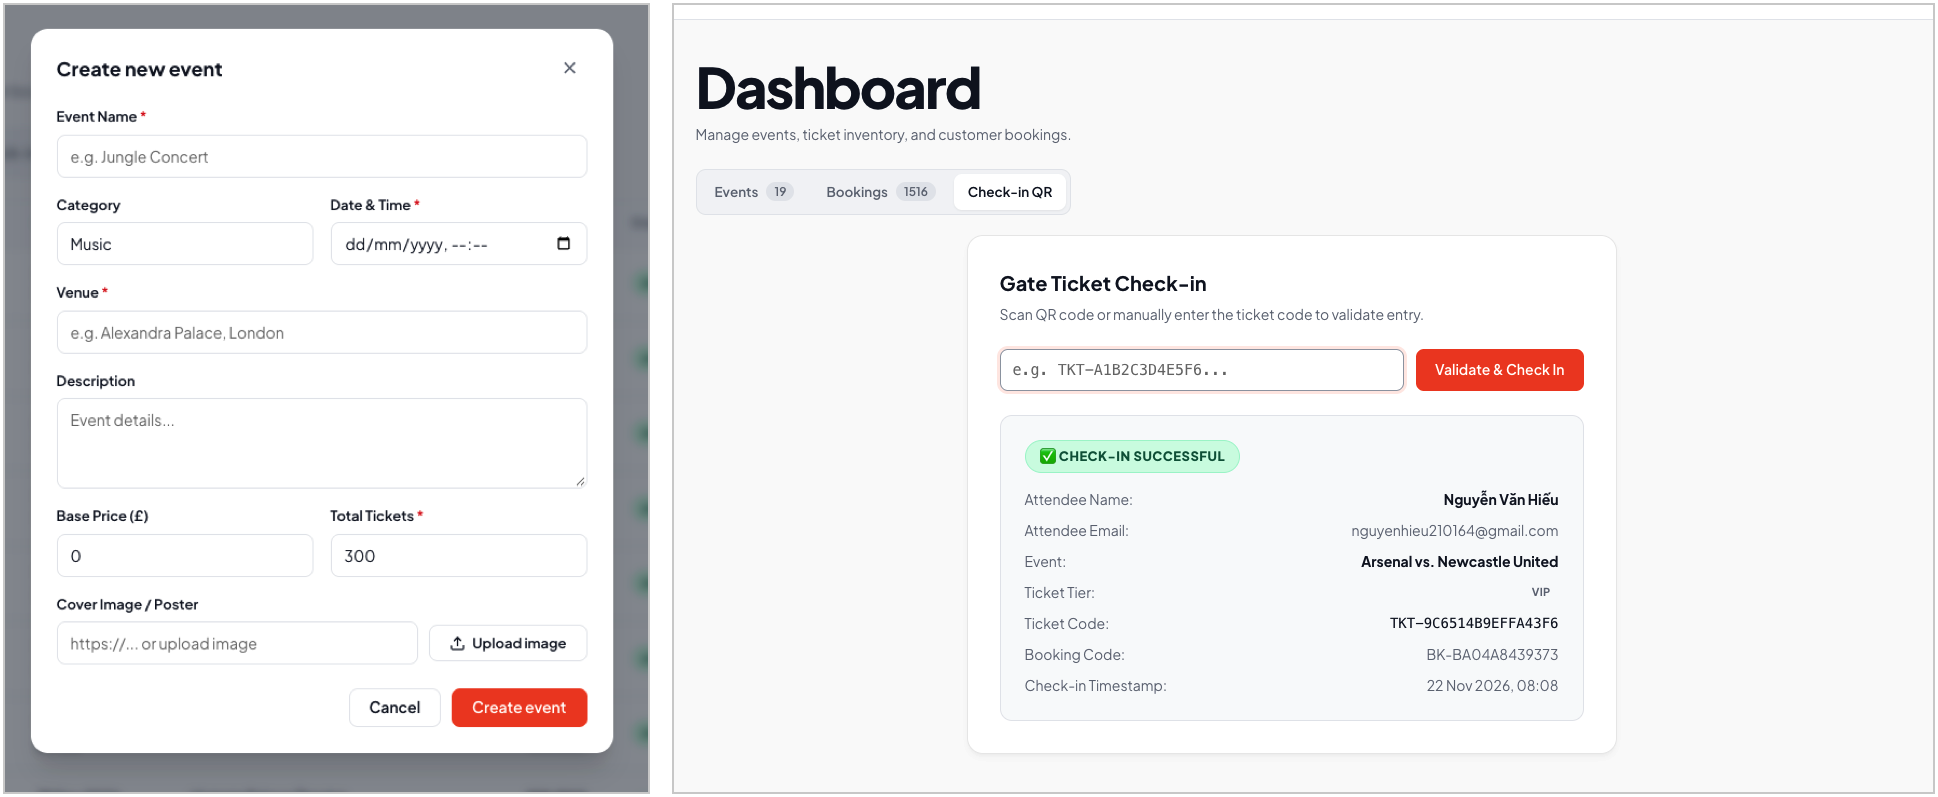
\includegraphics[width=\textwidth,height=0.31\textheight,keepaspectratio]{images/admin_checkin_qr.png}\\[2pt]
    {\tiny Admin Dashboard: Tải poster S3 \& Soát vé Check-in QR}

    \column{0.49\textwidth}
    \centering
    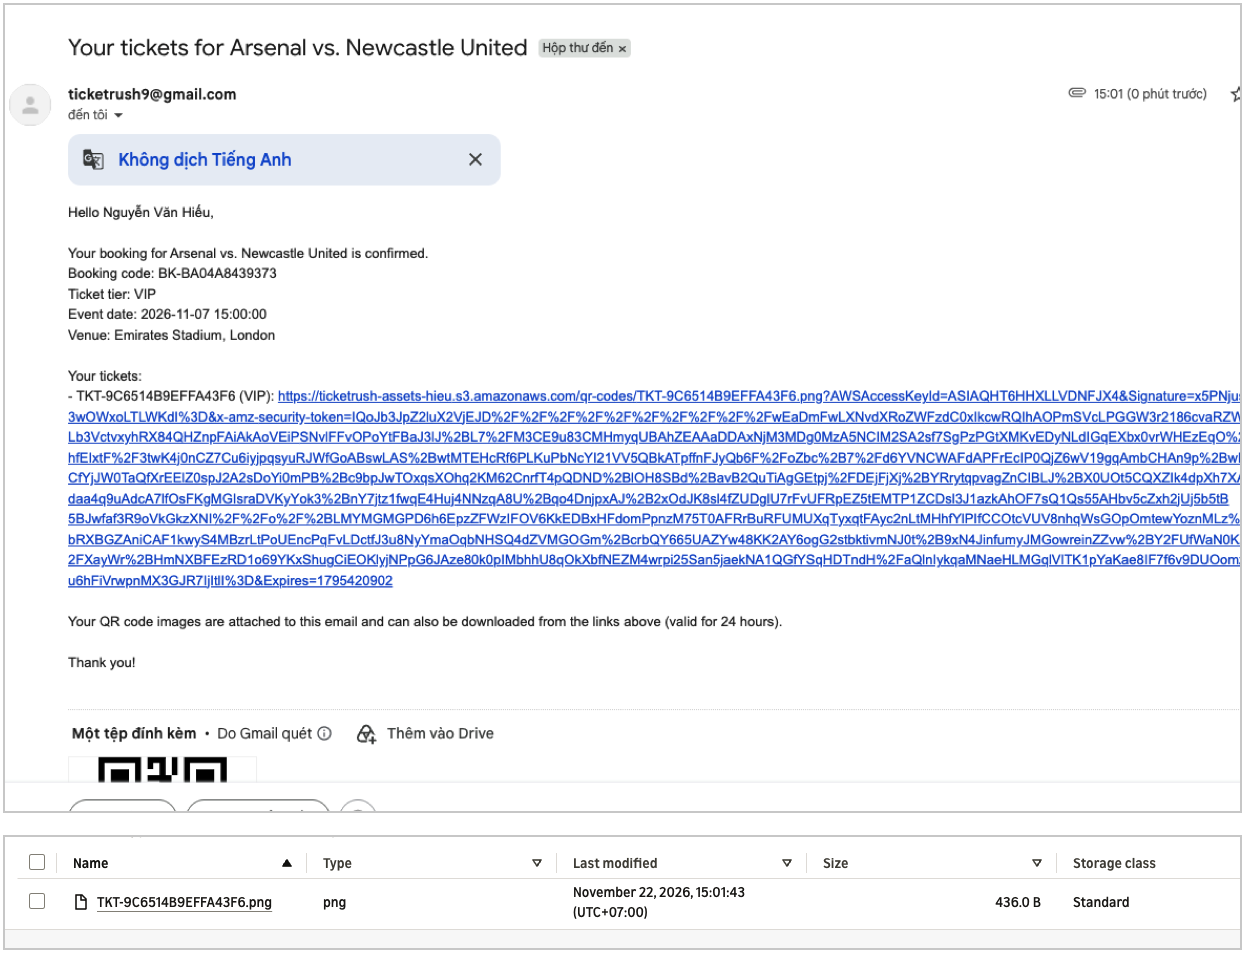
\includegraphics[width=\textwidth,height=0.68\textheight,keepaspectratio]{images/email_qr_s3.png}\\[2pt]
    {\tiny Email xác nhận kèm ảnh QR đính kèm \& tệp QR trên S3}
  \end{columns}
\end{frame}

% ============================================================================
% SLIDE 14: GIÁM SÁT CLOUDWATCH DASHBOARD, ALARMS & SNS
% ============================================================================
\begin{frame}{12. Giám sát CloudWatch Dashboard, 7 Alarms \& Amazon SNS}
  \begin{columns}[c]
    \column{0.52\textwidth}
    \centering
    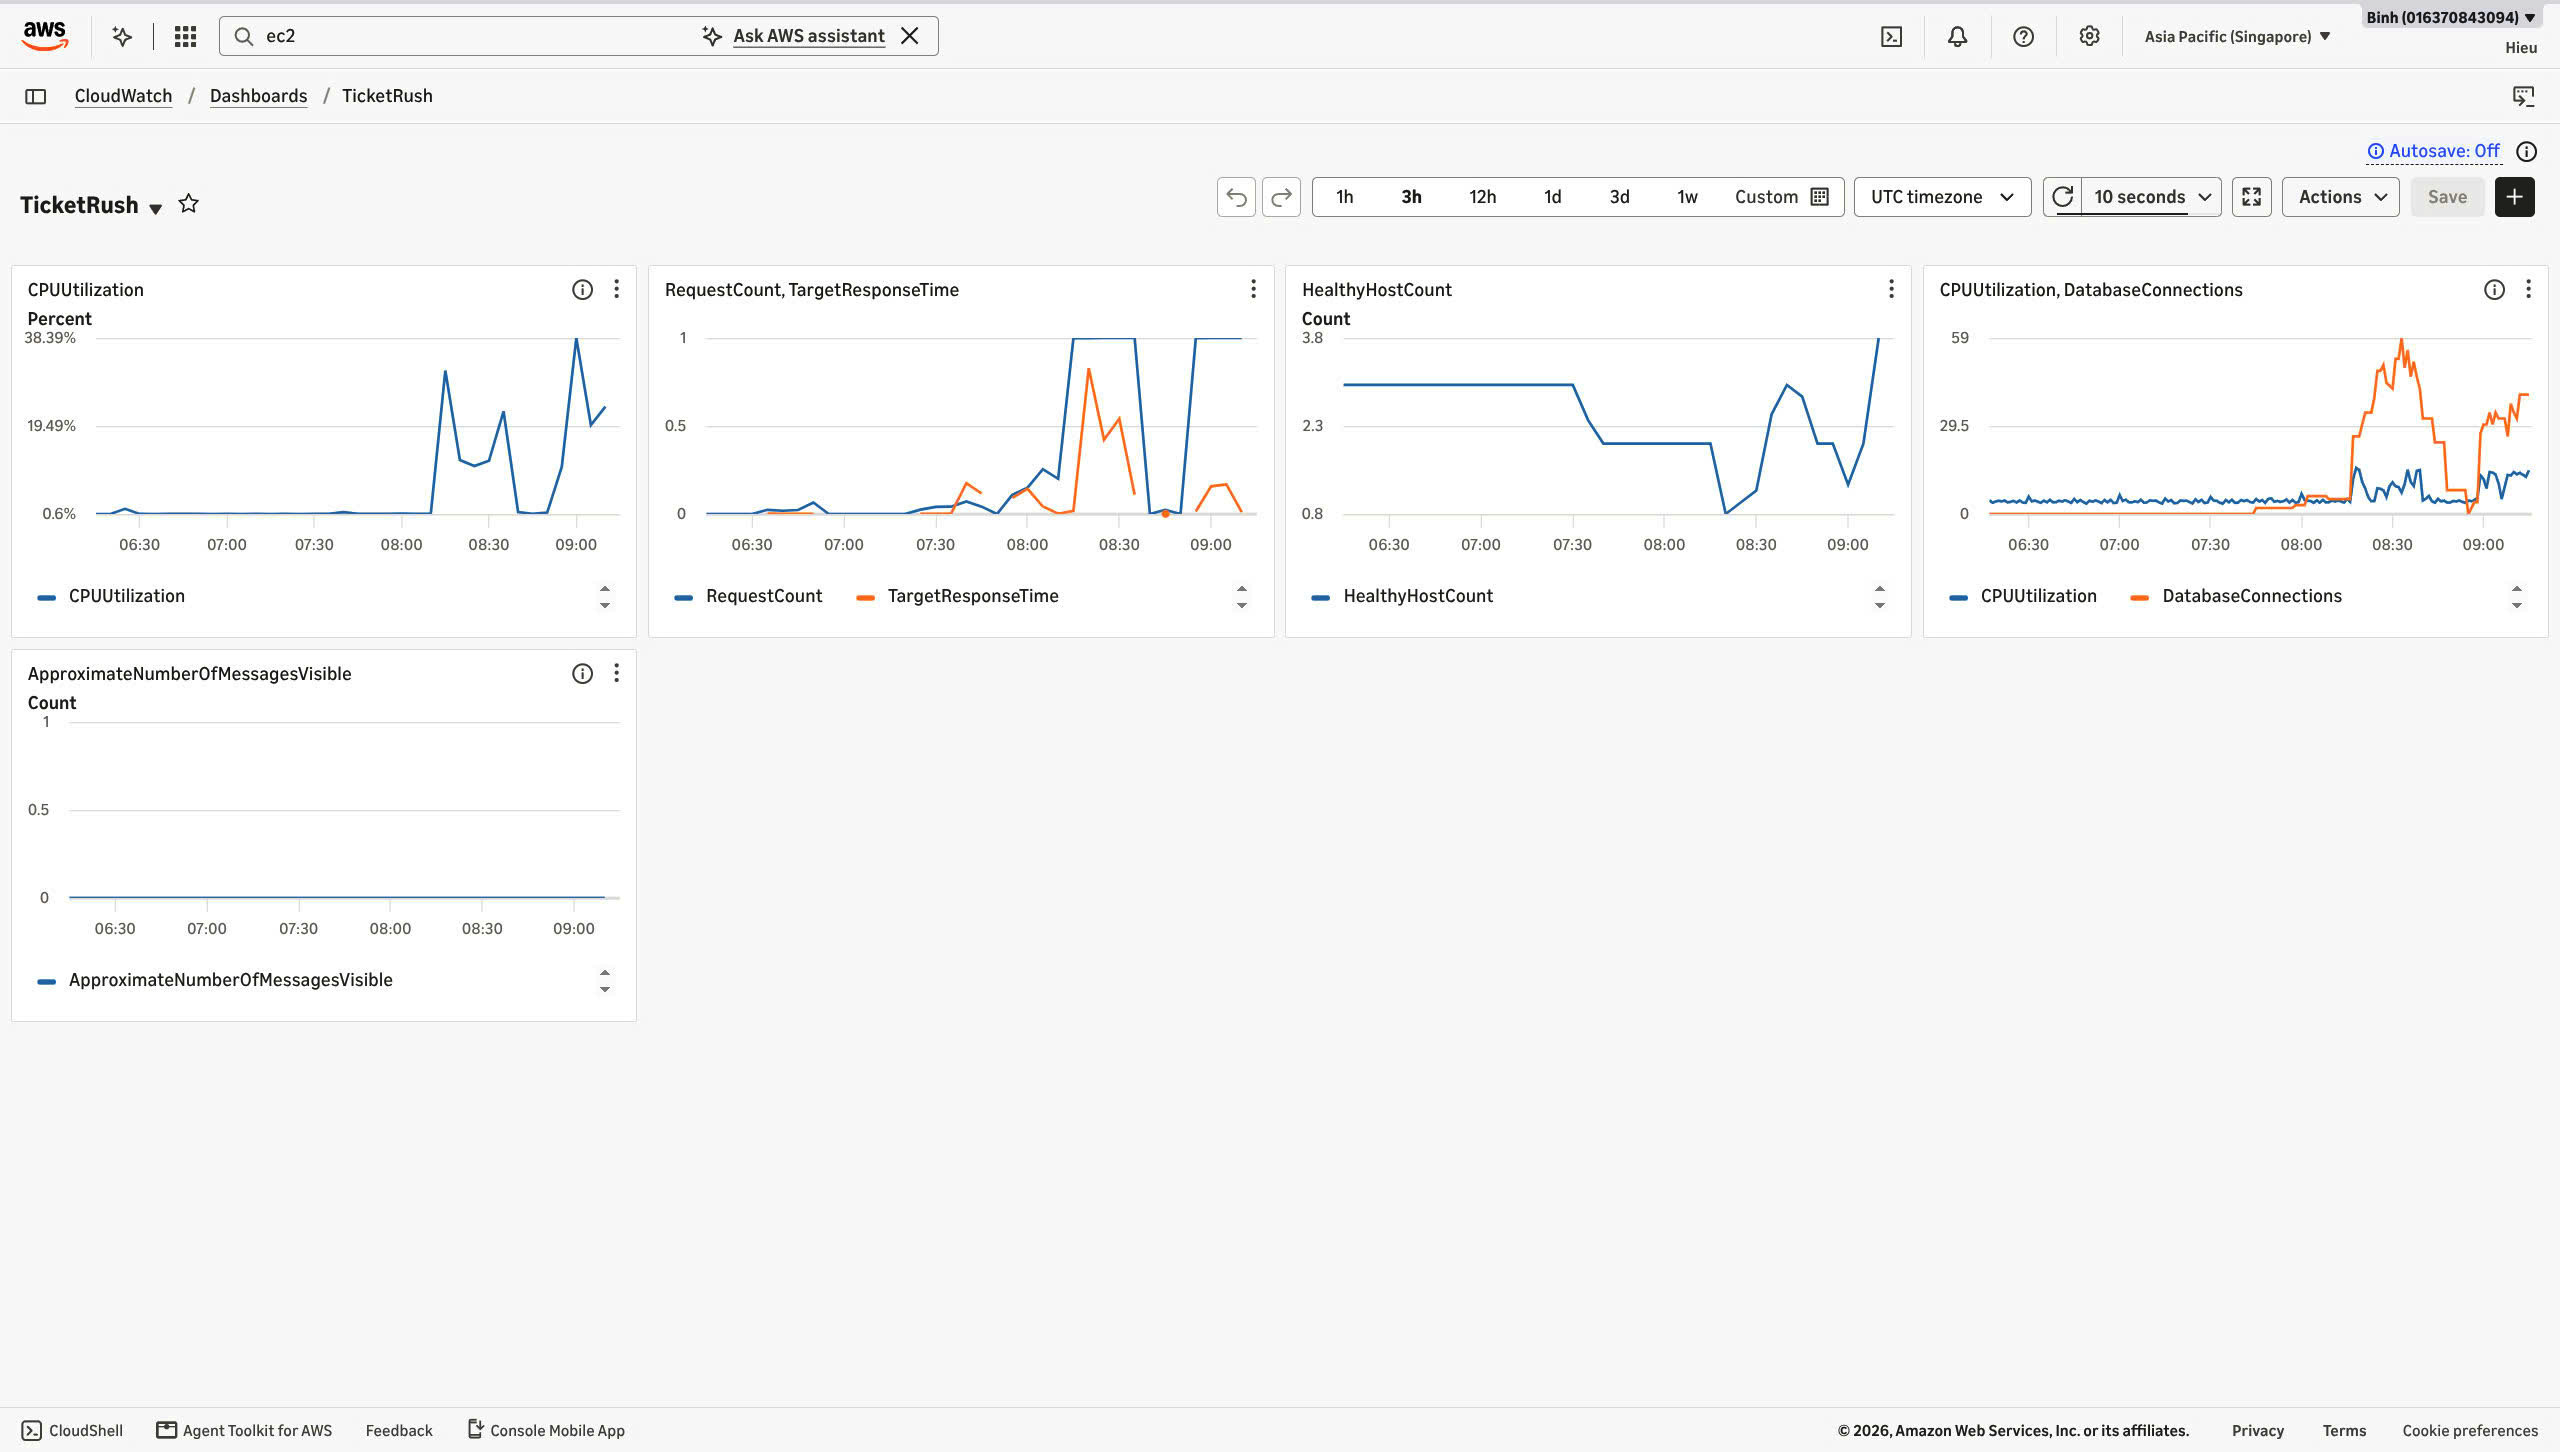
\includegraphics[width=\textwidth,height=0.52\textheight,keepaspectratio]{images/cloudwatch_dashboard.png}\\[4pt]
    \begin{beamercolorbox}[wd=\textwidth,rounded=true,sep=5pt]{block body}
      \scriptsize
      \textbf{CloudWatch Dashboard \texttt{TicketRush}:} Theo dõi đồng thời \texttt{EC2 CPU} (đỉnh 38,39\%), \texttt{ALB RequestCount/ResponseTime}, \texttt{HealthyHostCount} (lên 4), \texttt{RDS DatabaseConnections} và \texttt{SQS DLQ}.
    \end{beamercolorbox}

    \column{0.46\textwidth}
    \centering
    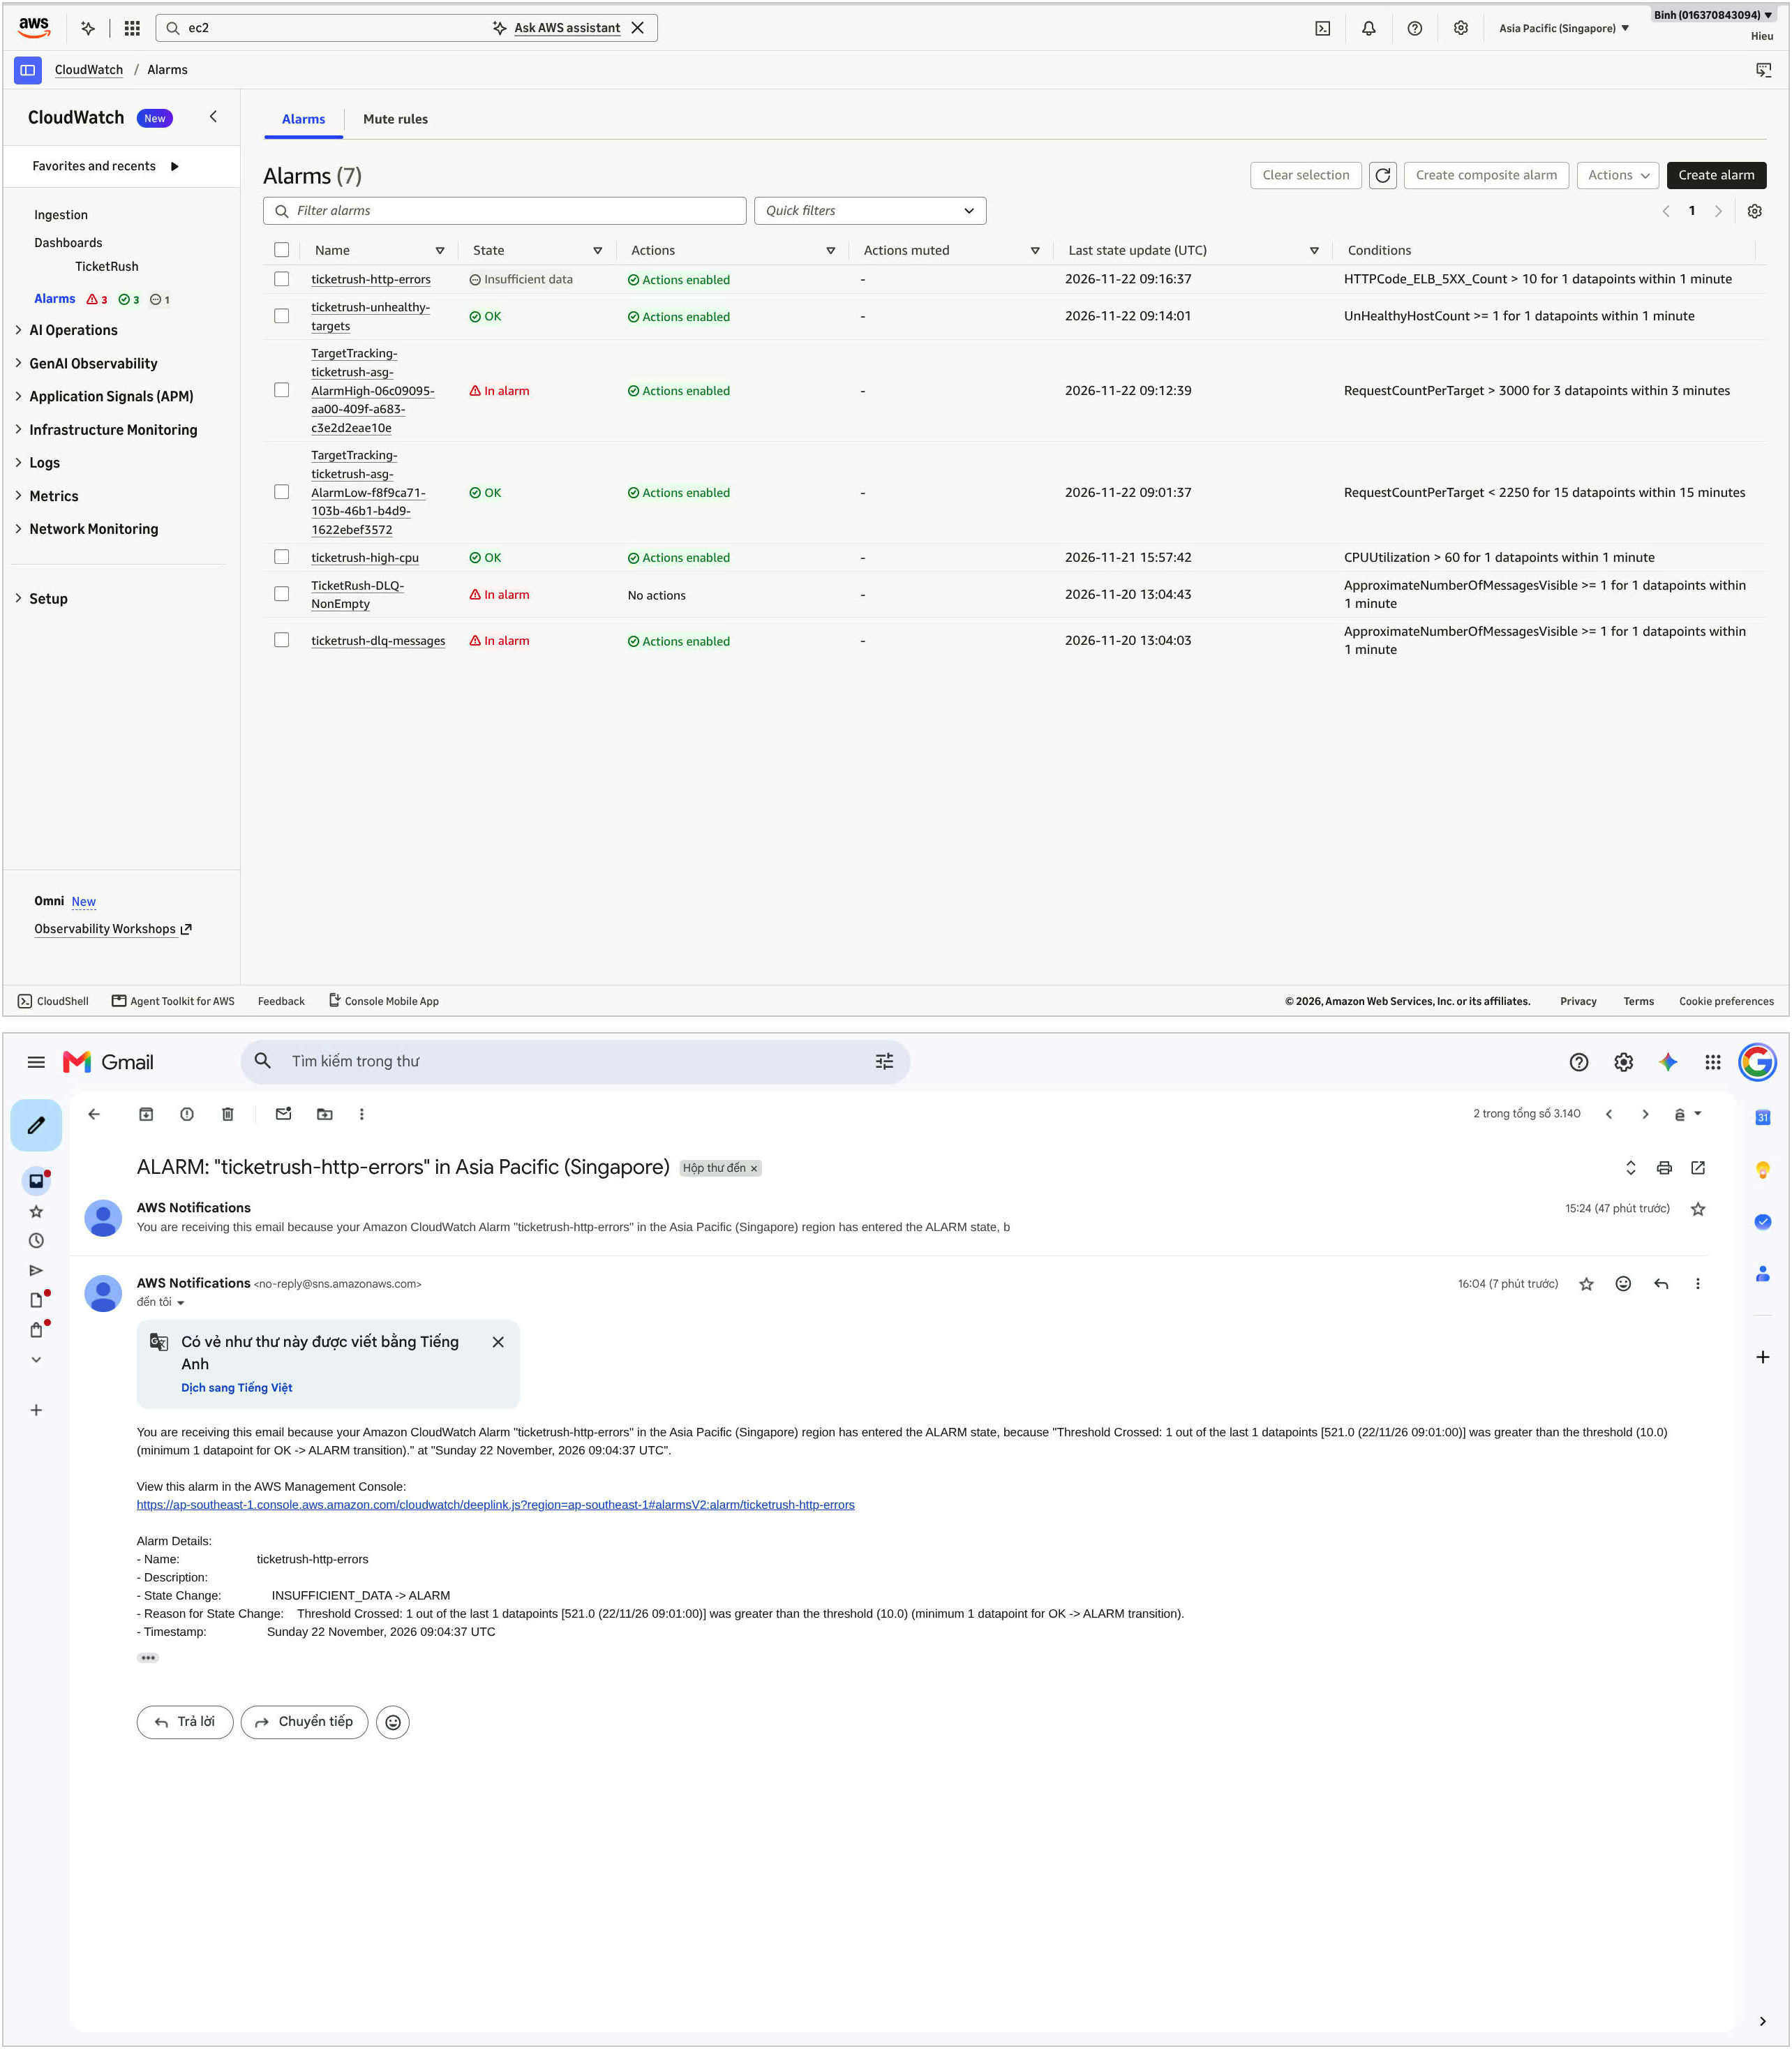
\includegraphics[width=\textwidth,height=0.75\textheight,keepaspectratio]{images/cloudwatch_alarms_sns.png}
  \end{columns}
\end{frame}

% ============================================================================
% SLIDE 15: KẾT QUẢ KIỂM THỬ CHỊU TẢI LOCUST (600 USERS)
% ============================================================================
\begin{frame}{13. Kết quả kiểm thử chịu tải thực tế (Locust - 600 Users)}
  \begin{columns}[c]
    \column{0.42\textwidth}
    \footnotesize
    \begin{itemize}
      \setlength{\itemsep}{4pt}
      \item \textbf{Kịch bản:} 600 users chạy liên tục $\sim$20 phút (\texttt{15:58 - 16:19}), gom tải vào sự kiện \#22 (300 chỗ).
      \item \textbf{Tổng lưu lượng:} \textbf{455.250 requests} (227.375 lượt đặt vé, 182.284 lượt xem sự kiện).
      \item \textbf{Thông lượng ổn định:} \textbf{289,1 - 291 RPS}.
      \item \textbf{Độ trễ cực thấp:}
        \begin{itemize}\scriptsize
          \item Tổng hợp: \textbf{Median 63 ms}, \textbf{p95 130 ms}, \textbf{p99 290 ms}.
          \item Đọc sự kiện (Redis Cache): \textbf{56 - 58 ms}.
        \end{itemize}
      \item \textbf{Tỉ lệ lỗi tổng:} Chỉ \textbf{0,41\%} (\textbf{0 lỗi/giây} liên tục >10 phút sau khi lên 4 EC2).
    \end{itemize}

    \column{0.56\textwidth}
    \centering
    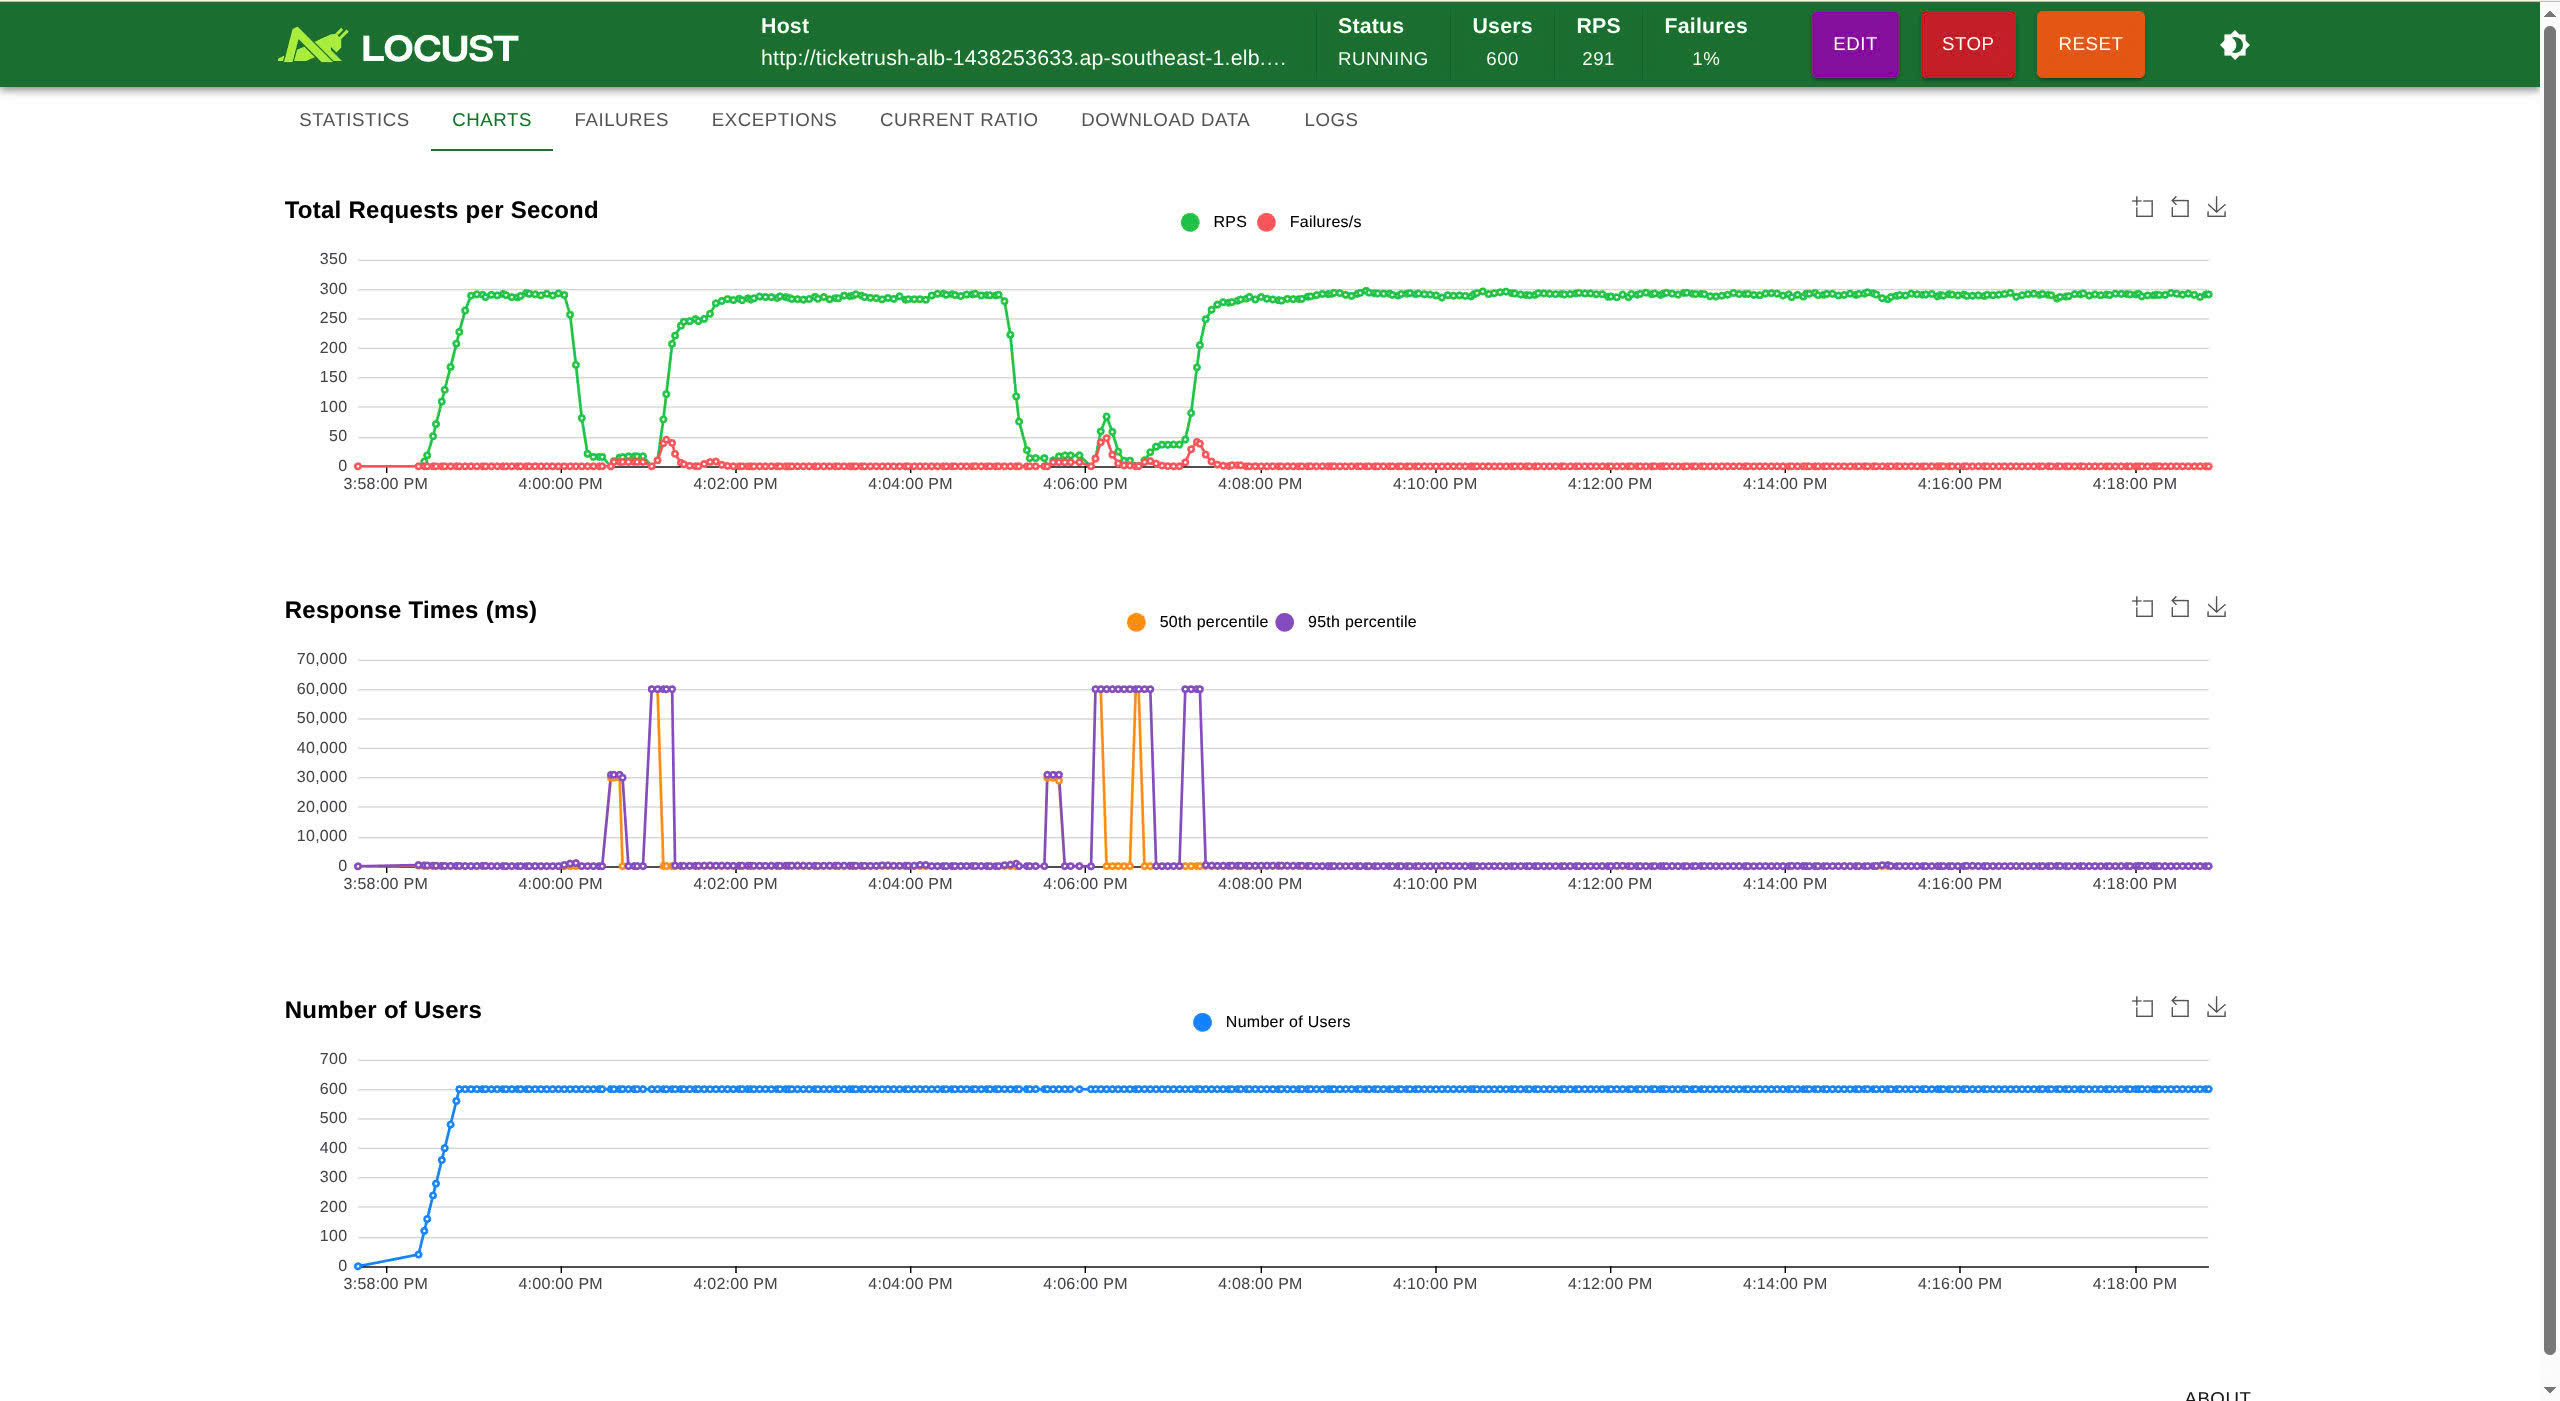
\includegraphics[width=\textwidth,height=0.74\textheight,keepaspectratio]{images/locust_charts.png}\\[3pt]
    {\scriptsize Biểu đồ Locust 600 users: phẳng tuyệt đối ở 291 RPS \& 0 lỗi/s từ 16:07:55}
  \end{columns}
\end{frame}

% ============================================================================
% SLIDE 16: AUTO SCALING, SELF-HEALING & CHỐNG BÁN LỐ 300/300
% ============================================================================
\begin{frame}{14. Minh chứng Auto Scaling, Self-Healing \& Chống bán lố}
  \begin{columns}[c]
    \column{0.44\textwidth}
    \scriptsize
    \begin{itemize}
      \setlength{\itemsep}{2.5pt}
      \item \textbf{Auto Scaling (2 $\rightarrow$ 4 EC2 trong 65s):}
        \begin{itemize}\scriptsize
          \item \texttt{AlarmHigh} kích hoạt policy \texttt{ticketrush-alb-request-tracking} lúc \texttt{16:06:50}.
          \item 2 máy mới sẵn sàng lúc \texttt{16:07:55} (chỉ \textbf{65 giây} nhờ Golden AMI).
        \end{itemize}
      \item \textbf{Tự phục hồi (Self-Healing):}
        \begin{itemize}\scriptsize
          \item Lúc \texttt{16:10:12}, 1 node trượt ELB Health Check $\rightarrow$ Connection Draining êm ái \& tự launch máy thay thế trong \textbf{6 giây}.
        \end{itemize}
      \item \textbf{Kiểm chứng 300/300 vé (sự kiện \#22):}
        \begin{itemize}\scriptsize
          \item Admin Dashboard: \texttt{0/300 (100\% sold)}.
          \item RDS qua SSM: \texttt{[(22, 300, 0)]} \& \texttt{[(300, 300)]}.
        \end{itemize}
    \end{itemize}

    \column{0.54\textwidth}
    \centering
    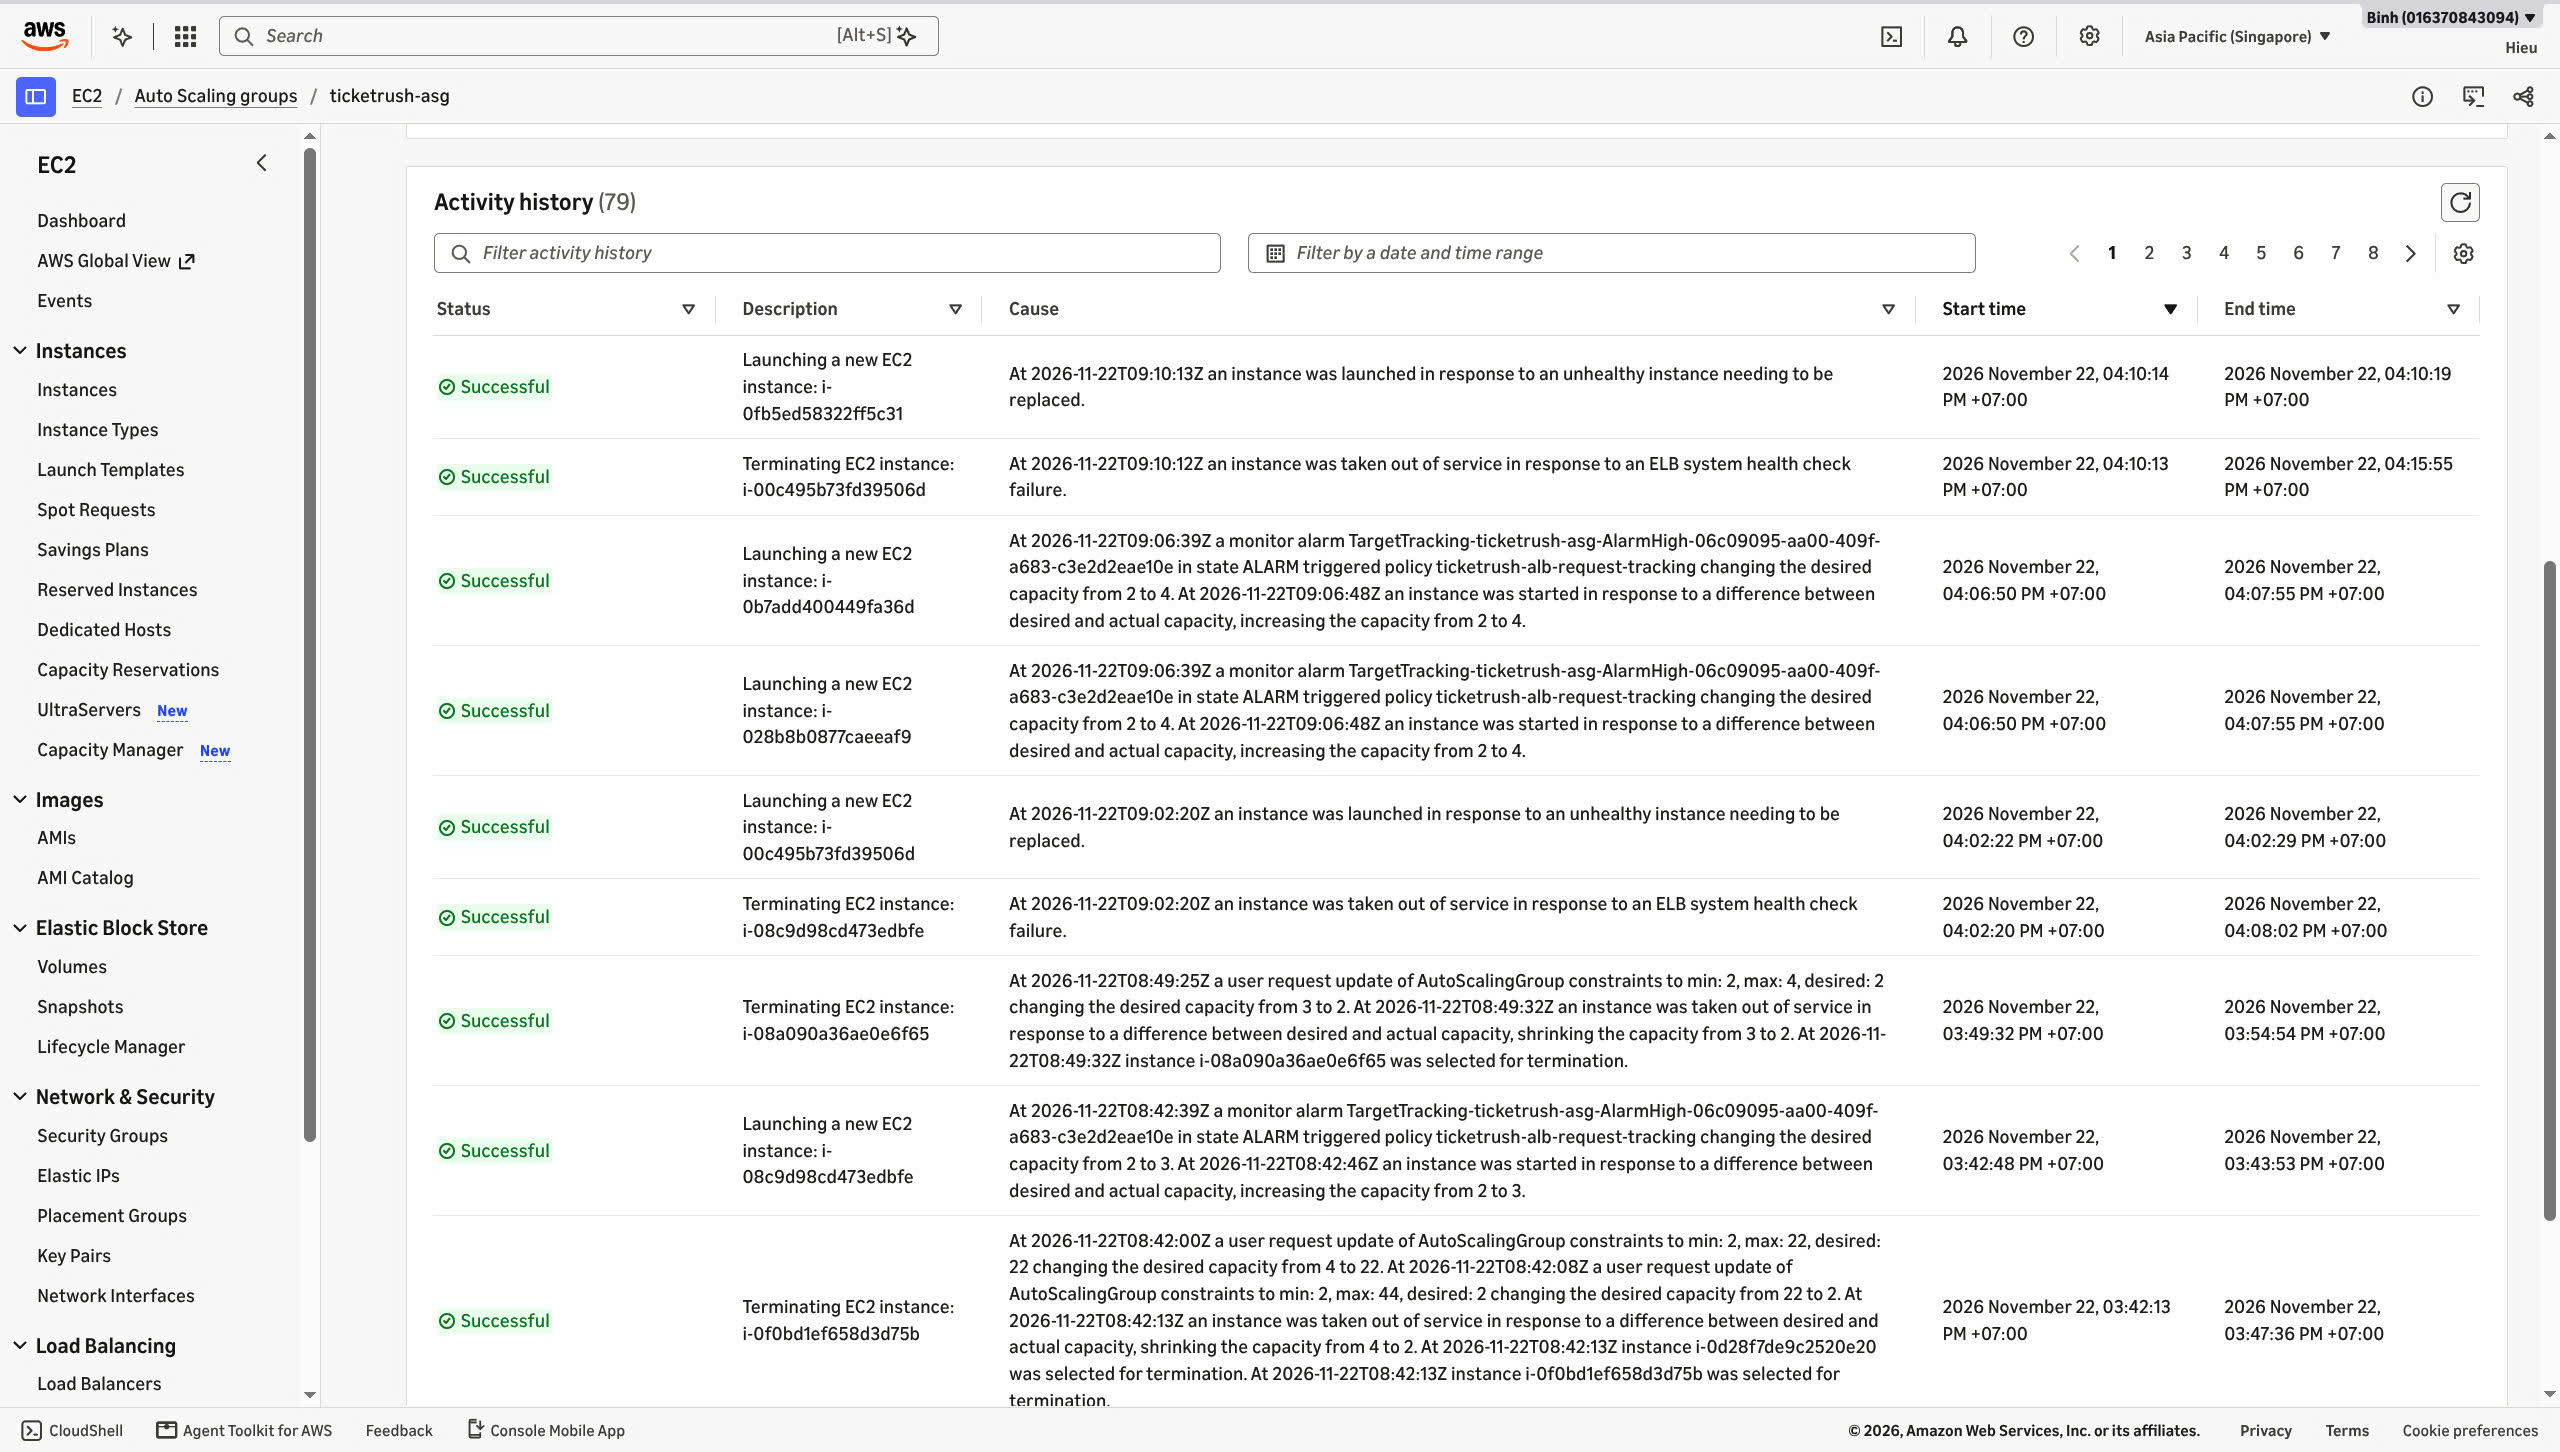
\includegraphics[width=\textwidth,height=0.50\textheight,keepaspectratio]{images/asg_activity_scaleout.png}\\[5pt]
    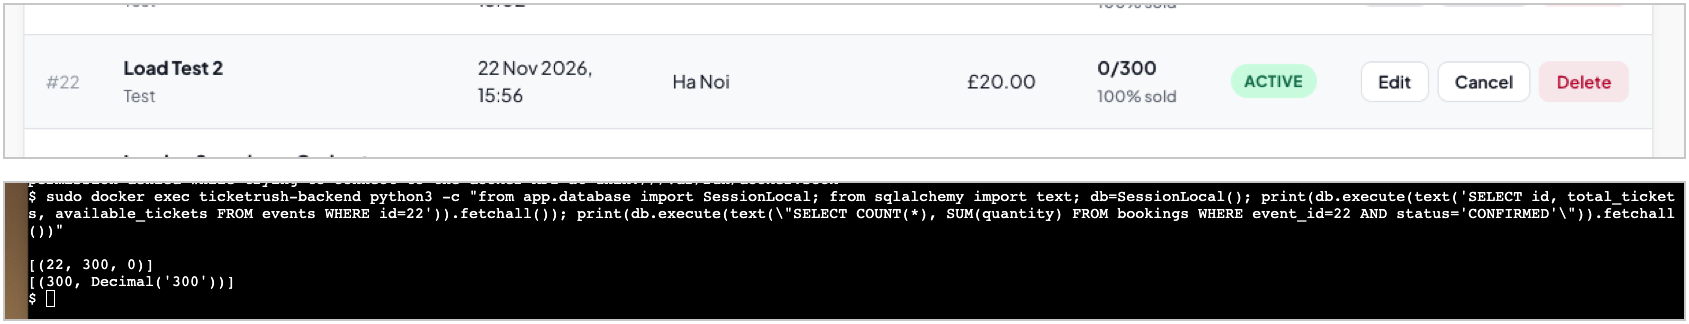
\includegraphics[width=\textwidth,height=0.22\textheight,keepaspectratio]{images/dbeaver_300_tickets.png}
  \end{columns}
\end{frame}

% ============================================================================
% SLIDE 17: CHI PHÍ VẬN HÀNH & LÝ DO LỰA CHỌN CÔNG NGHỆ
% ============================================================================
\begin{frame}{15. Ước tính chi phí hàng tháng \& Lý do lựa chọn công nghệ}
  \begin{columns}[T]
    \column{0.49\textwidth}
    \textbf{\small Ước tính chi phí 24/7 (\texttt{ap-southeast-1}):}
    \vspace{5pt}
    {\scriptsize
    \renewcommand{\arraystretch}{1.22}
    \begin{tabular}{@{} >{\raggedright\arraybackslash}p{4.3cm} r @{}}
      \toprule
      \textbf{Thành phần AWS} & \textbf{USD/tháng} \\
      \midrule
      NAT Gateway (1 AZ + lưu lượng) & \$48.00 \\
      RDS MySQL \texttt{db.t3.micro} Multi-AZ & \$42.00 \\
      EC2 \texttt{t3.small} $\times$ 2 máy + EBS & \$43.00 \\
      ALB (24/7) + IPv4 \& Data Out & \$39.00 \\
      ElastiCache Redis \texttt{cache.t3.micro} & \$15.00 \\
      CW/SNS, S3, SQS, Lambda, CF, DDB & \$9 - \$11 \\
      \midrule
      \textbf{Tổng ước tính hàng tháng} & \textbf{$\approx$ \$196 - \$198} \\
      \bottomrule
    \end{tabular}
    }

    \column{0.48\textwidth}
    \begin{block}{Lý do lựa chọn công nghệ chính}
      \footnotesize
      \begin{itemize}
        \setlength{\itemsep}{3pt}
        \item \textbf{RequestCount vs CPU:} Web I/O-bound nên \texttt{ALBRequestCountPerTarget} mở rộng kịp thời khi CPU mới ở 38,39\%.
        \item \textbf{Golden AMI:} Máy mới sẵn sàng sau 65s thay vì 4-5 phút build lại lúc boot.
        \item \textbf{Redis + RDS Multi-AZ:} Vừa nhanh trên RAM vừa đảm bảo ACID, chống bán lố tuyệt đối.
        \item \textbf{Tối ưu chi phí:} Auto scale-in về 2 EC2, tắt Bastion khi không dùng, CloudFront Free Tier.
      \end{itemize}
    \end{block}
  \end{columns}
\end{frame}

% ============================================================================
% SLIDE 18: CẢM ƠN & DEMO
% ============================================================================
\begin{frame}
  \centering
  \vspace*{0.8cm}
  {\Huge\color{uetblue} Cảm ơn thầy cô đã lắng nghe!}\\[0.5cm]
  {\large Q\&A \& Demo trực tiếp hệ thống}\\[0.7cm]
  \begin{block}{Thông tin truy cập hệ thống}
    \centering\small
    \textbf{Hệ thống triển khai:} \url{https://d3m6e24vu2nkwf.cloudfront.net}\\[4pt]
    \textbf{Trang quản trị:} \url{https://d3m6e24vu2nkwf.cloudfront.net/admin.html}\\[4pt]
    \textbf{Mã nguồn GitHub:} \url{https://github.com/nguyenhieu21016/TicketRush}
  \end{block}
\end{frame}

\end{document}
